% !Mode:: "TeX:UTF-8"
% !TEX program  = xelatex

\documentclass[bwprint]{gmcmthesis}
% \documentclass[bwprint,fontset=fandol]{gmcmthesis} % Overleaf 等在线平台需要用这一行。
\usepackage[framemethod=TikZ]{mdframed}
\usepackage{amssymb}
\usepackage{dsfont}

\usepackage{subfig}
\usepackage{colortbl}
\usepackage{threeparttable}
\DeclareMathOperator{\clip}{clip}
\providecommand{\I}{\mathds{1}}
\providecommand{\E}{\mathbb{E}}
\definecolor{color2}{rgb}{0.36,0.62,0.84}
% \definecolor{color3}{rgb}{0.8235,0.8706,0.9373}
\definecolor{color3}{rgb}{0.88,0.92,0.96}
\definecolor{color4}{rgb}{0.96,0.97,0.98}   % {0.9176,0.9373,0.9686}

% 算法
\usepackage[noend]{algpseudocode}
\usepackage{algorithmicx,algorithm}
\floatname{algorithm}{算法}
\renewcommand{\algorithmicrequire}{\textbf{输入:}}
\renewcommand{\algorithmicensure}{\textbf{输出:}}
% \numberwithin{equation}{section}
% \numberwithin{figure}{section}
% \numberwithin{table}{section}
\newcommand{\red}[1]{\textcolor{red}{#1}}
\newcommand{\blue}[1]{\textcolor{blue}{#1}}


\title{算力约束下提升大语言模型能力的资源配置建模}   % 标题
\baominghao{26102860508}   % 参赛队号
\schoolname{东南大学}   % 学校名称(跨校加角标$^1$标注对应关系)
\membera{杨嘉诚}   % 队员A(跨校加角标$^1$标注对应关系)
\memberb{李邵恺}   % 队员B(跨校加角标$^1$标注对应关系)
\memberc{许圣炜}   % 队员C(跨校加角标$^1$标注对应关系)
\begin{document}

% 生成标题
\maketitle


\begin{abstract}    % 摘要
    数学建模
    \keywords{模板\quad  \LaTeX{}\quad   数学建模}    % 关键字
\end{abstract}

\pagestyle{plain}

\tableofcontents    % 目录


\section{问题重述}  % 1
\textbf{问题一：}

附件 A 给出两类数据。

第一类为 A1--A3 的质量信号数据，每条文本包含 22 个质量指标，其中既有教育价值、流畅度、可读性等正向指标，也有广告概率、重复比例等负向指标，还有文本长度、数字比例等不宜简单假定单调优劣的指标。题目要求使用 A1 抽样集以及 A2、A3 扩展集的全部记录，建立样本级和领域级质量评分 $Q$，并检验扩展集与抽样集是否具有一致结论。当不同指标对同一文本给出显著不一致的判断时，还需定义冲突、分析来源并提出消解方法。

第二类为 A4--A15 的 RegMix 配方实验数据。每个配方由 17 个 The Pile 子领域的份额构成，份额非负且和为 1；对应结果为 13 个验证领域的交叉熵 Loss。需要利用 A4/A5 建模，在 A6--A11 的 1M、60M、1B 检验集上验证，并利用 A12--A15 讨论 10B 和 70B 外推结论的稳健性。由于质量信号领域和配方领域并不完全一致，若将 $Q$ 引入配比模型，必须说明映射、可辨识性和不确定性。

\textbf{问题二：}

在问题一得到的质量评分与领域配比模型基础上，结合附件 B 的参数规模、训练数据量、质量和 Loss 数据，建立能够同时描述 $N$、$D$、$Q$ 与 $\bm p$ 影响的广义标度律。模型应在参考质量和参考配比条件下退化为经典标度律，并说明不同来源数据的衔接方式与质量响应系数 $\gamma$ 的可识别条件。

需要通过规模留出、训练阶段留出和按 \((N,D)\) 组合分组的质量模型交叉验证，区分真实记录、半合成、插值及估算数据的证据性质；进一步求解参数量、数据量和质量的边际收益，给出质量提高与参数扩容达到同等性能时的替代条件，并分析领域配比的局部互补或替代关系。对缺少实际成本和联合实验的数据条件，采用条件分析与敏感性分析界定结论范围。


\section{模型假设}  % 2
\begin{enumerate}[label=\textbf{H\arabic*.},leftmargin=2.5em]
    \item 附件中标记为真实的数据能够代表对应数据源；半合成、子集和外推数据按其标记使用，不与真实实验混同。
    \item 二分类列表的末位为正类 logits，ModernBERT 六维输出的类别顺序与质量等级一致；若原始模型标签顺序相反，应在代码配置中同步调整。
    \item A1 可作为 22 个质量指标归一化和权重估计的参考样本，A2/A3 只用于扩展验证和相应领域最终评分。
    \item 配比表中的舍入误差可通过闭合操作修正；加入小伪计数后，零份额的对数比可以稳定计算。
    \item 二次响应面只解释观测配方邻域内的关联效应，有限差分不被解释为全局因果效应。
    \item 不同参数规模改变绝对 Loss 基准，但配方优劣排序可能迁移，因此跨规模以秩相关为主要评价标准。
    
    \item 同一评价口径下，参数受限与数据受限造成的超额 Loss 可用正系数双幂律近似；不同来源允许具有不同的基线系数。
    \item 固定领域配比时，额外质量改善使超额 Loss 按比例变化。质量响应由 B6 的半合成记录条件估计，其迁移到基准模型的有效性需要分层检验。
    \item 问题一的质量代表值只用于构造常规质量基准，未映射领域仍保留条件区间；问题一已拟合的配比响应包含原有语料条件下的质量差异，不重复计算其贡献。
    \item 主情景的质量尺度换算系数 $\kappa$ 和配比迁移强度取 $\kappa=\lambda_p=1$。二者并非现有数据唯一识别的参数，其变化通过敏感性分析报告。
    
\end{enumerate}


\section{定义与符号说明}   % 3
\begin{table}[H]    % table 3.1
    \centering
    \caption{主要符号}
    \label{tab:symbols}
    \begin{tabularx}{0.92\textwidth}{cX}
        \toprule
        符号 & 含义 \\
        \midrule
        $i,j,d,k,r,s$ & 文本、质量指标、质量领域、配方领域、Loss 验证域、模型规模的下标 \\
        $x_{ij}$ & 列表压缩后的原始质量指标 \\
        $S_{ij}$ & 方向统一后的质量得分，取值在 $[0,1]$ \\
        $w_j$ & 第 $j$ 个质量指标的受限 CRITIC 权重 \\
        $Q_i,Q_d$ & 文本级综合质量与领域级质量 \\
        $D_i,R_i$ & 文本的加权分歧度与 90\%--10\% 稳健极差 \\
        $Conf_i$ & 文本质量评分置信度 \\
        $\bm p_i$ & 17 维领域配比，满足非负且和为 1 \\
        $\bm z_i$ & 配比的 16 维 ILR 坐标 \\
        $L_{ir},\widehat L_{ir}$ & 观测和预测的第 $r$ 个验证域 Loss \\
        $ME_k,INT_{jk}$ & 领域边际效应和两领域二阶组合效应 \\

        $N,D$ & 模型参数个数与训练 token 数 \\
        $n,d$ & 归一化规模，$n=N/10^9$、$d=D/10^{11}$ \\
        $Q,\bar Q(\bm p)$ & 当前语料质量与配方的常规质量基准 \\
        $\bm p_0,Q_0$ & 参考配比与参考质量，$Q_0=\bar Q(\bm p_0)$ \\
        $f_A(\bm p),h(\bm p)$ & 问题一对13个验证领域的平均预测 Loss 及其对数相对响应 \\
        $E,A,B,\alpha,\beta$ & 渐近 Loss、规模项幅度及衰减指数 \\
        $\gamma,\kappa$ & 质量响应系数与质量量尺换算系数 \\
        $\lambda_p$ & 配比迁移强度，与问题一岭惩罚 $\lambda$ 区分 \\
        $G(Q,\bm p)$ & 质量和配比的乘性修正因子 \\
        $X,Y$ & 参数受限项 $An^{-\alpha}$ 与数据受限项 $Bd^{-\beta}$ \\
        $\omega_i$ & 问题二拟合记录的均衡权重 \\
        $U_n,U_d,U_Q$ & 单位规模、数据量及质量的边际降损收益 \\
        $c_n,c_Q$ & 单位归一化参数量及质量的边际成本 \\
        $N_{\mathrm{eq}},\Delta Q$ & 等效参数量与质量的绝对提高量 \\
        $I_{jk},\varepsilon_p$ & 参考点领域混合导数与份额差分步长 \\
        
        \bottomrule
    \end{tabularx}
\end{table}


\section{问题一}   % 4
    \subsection{问题分析}   % 4.1
    质量信号的主要困难不是简单加权，而是输出结构和语义不同。二分类模型输出 logits，有序分类器输出 6 维 logits，Qurater 给出多个并列质量侧面\textsuperscript{\cite{wettig2024qurating}}，而 RedPajama 统计量为连续标量。若直接对列表取均值，会混淆概率、等级和不同侧面的含义。其次，``词数越多越好''或``数字比例越低越好''并不适用于所有领域，必须将这类指标视为目标型而非强行设定单调方向。最后，扩展集中 arxiv 和 github 的记录数远大于其他领域，若直接用全体数据估计权重，会让领域规模影响指标权重。因此本文只用覆盖 7 个领域的 A1 估计归一化参数和权重，再把同一变换应用到 A2/A3。

    质量指标的分歧可能来自真实的多面性，也可能来自分类器误差、文本格式或极端长度。仅用最大值减最小值会被单项异常放大，仅用方差又可能把多个指标的系统性对立平均掉。本文联合使用加权分歧度和 90\%--10\% 稳健极差，并以 A1 分歧度的高分位数确定阈值。综合评分借鉴 Huber 鲁棒估计\textsuperscript{\cite{huber1964robust}}，使冲突记录中的离群指标自动降权，而不是删除整条文本。

    17 个领域份额属于成分数据。在含截距的回归中同时纳入全部原始份额会产生完全共线性，成分数据分析强调以分量间的相对比例刻画其变化\textsuperscript{\cite{aitchison1982compositional}}。同时，13 个验证域的 Loss 相关但不完全相同，需要多输出建模。RegMix 将数据配比优化转化为性能回归预测，并检验小模型配方排序向较大模型迁移的效果\textsuperscript{\cite{liu2025regmix}}。本题 RegMix 的训练表只有 512 个配方，若使用高复杂度黑箱模型，不利于效应解释且容易过拟合。本文采用 ILR 坐标上的二次岭回归：ILR 将配比映射到正交的对数比坐标\textsuperscript{\cite{egozcue2003ilr}}，二次项表达组合关系，岭惩罚用于降低共线性带来的估计不稳定性\textsuperscript{\cite{hoerl1970ridge}}。

    \begin{figure}[H]
      \centering
      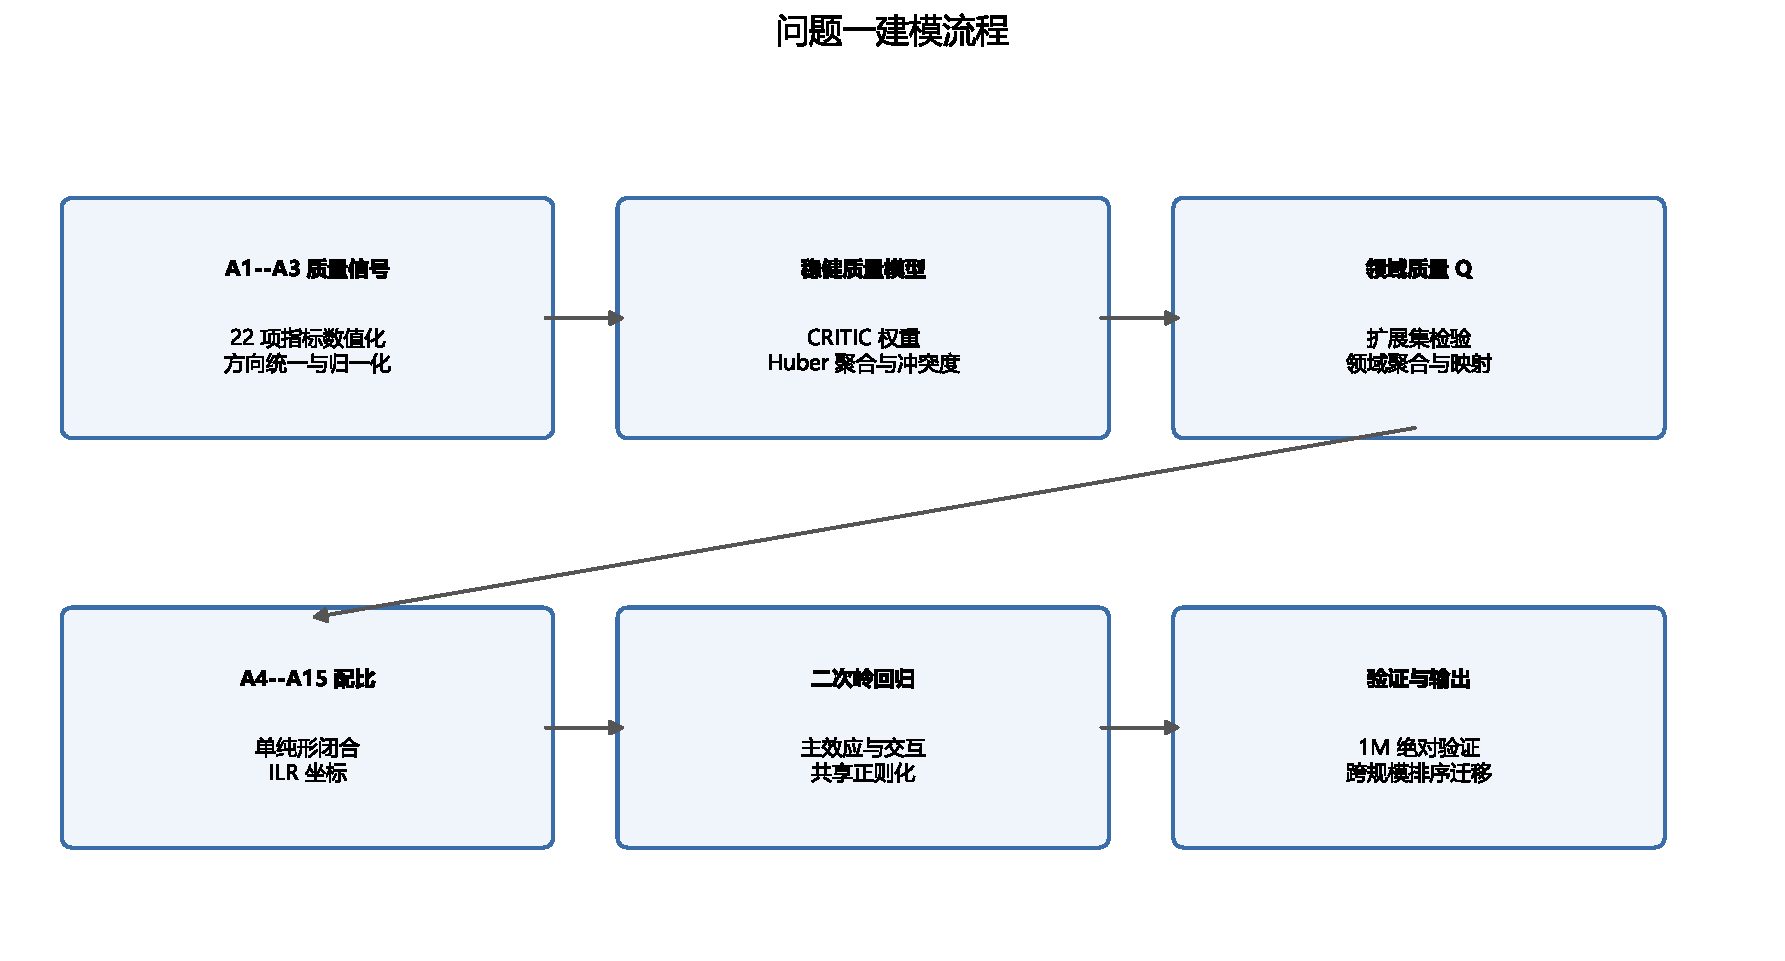
\includegraphics[width=0.96\textwidth]{figures/q1_fig01_modeling_workflow.pdf}   % figure 4.1
      \caption{问题一建模流程 (待更新)}
      \label{fig:workflow}
    \end{figure}
    
    \subsection{模型建立}   % 4.2
        \subsubsection{列表型质量信号标量化}  % 4.2.1 
        设文本 $i$ 的指标 $j$ 原始输出为 $x_{ij}$。标量字段直接保留；8 个列表型字段按输出含义处理。

        对 `fluency\_en' 和 `ad\_en' 的二分类 logits $(a_0,a_1)$，取正类概率：
        \begin{equation}
        x_{ij}=\frac{\exp(a_1)}{\exp(a_0)+\exp(a_1)}.
        \label{eq:binary}
        \end{equation}
        
        对四个 `modernbert\_*' 的 6 级有序 logits，取归一化期望等级：
        \begin{equation}
        x_{ij}=\sum_{c=0}^{5}\frac{c}{5}
        \frac{\exp(a_c)}{\sum_{h=0}^{5}\exp(a_h)}.
        \label{eq:ordinal}
        \end{equation}
        
        `qurater' 的四个分量对应 QuRating 的并列质量侧面\textsuperscript{\cite{wettig2024qurating}}。本文在此基础上进行标量化，分别经逻辑函数后求平均：
        \begin{equation}
        x_{ij}=\frac{1}{4}\sum_{c=1}^{4}\frac{1}{1+\exp(-a_c)}.
        \label{eq:qurater}
        \end{equation}
        
        `fineweb\_edu' 的列表仅含一个元素，直接取其值。这样避免了对 logits 直接平均造成的量纲错误。


        \subsubsection{方向统一与缺失处理}   % 4.2.2 
        以 A1 为参考样本，计算指标 $j$ 的 1\%、50\%、99\% 分位数 $q_{.01,j},q_{.50,j},q_{.99,j}$，并将极端值缩尾到该区间。效益型指标转换为
        \begin{equation}
        S_{ij}=\frac{\clip(x_{ij})-q_{.01,j}}{q_{.99,j}-q_{.01,j}},
        \label{eq:benefit}
        \end{equation}
        成本型指标转换为
        \begin{equation}
        S_{ij}=1-\frac{\clip(x_{ij})-q_{.01,j}}{q_{.99,j}-q_{.01,j}}.
        \label{eq:cost}
        \end{equation}
        
        词数、句数、数字比例和平均词长设为目标型指标：
        \begin{equation}
        S_{ij}=\begin{cases}
        1-\dfrac{q_{.50,j}-x_{ij}}{q_{.50,j}-q_{.01,j}},&x_{ij}\le q_{.50,j},\\[6pt]
        1-\dfrac{x_{ij}-q_{.50,j}}{q_{.99,j}-q_{.50,j}},&x_{ij}>q_{.50,j}.
        \end{cases}
        \label{eq:target}
        \end{equation}
        所有结果截断到 $[0,1]$，从而统一为越高越好。缺失值先用同领域中位数填补，再用 A1 全局中位数兜底；另保留原始覆盖率，防止填补后的记录被误认为信息完整。
        
        
        \subsubsection{受限 CRITIC 权重}    % 4.2.3
        在方向统一后的 A1 得分上计算标准差 $\sigma_j$ 和相关系数 $\rho_{jh}$。经典 CRITIC 方法综合指标的变异性与冲突性确定客观权重\textsuperscript{\cite{diakoulaki1995critic}}。本文借鉴其赋权思想，将相关系数替换为绝对相关系数，以衡量正负相关所体现的信息冗余，定义改进信息量与权重为
        \begin{equation}
        C_j=\sigma_j\sum_{h=1}^{22}(1-|\rho_{jh}|),\qquad
        w_j^{(c)}=\frac{C_j}{\sum_hC_h}.
        \label{eq:critic}
        \end{equation}
        
        为避免噪声造成权重过度集中，将 CRITIC 权重与等权重各占一半，并限制单项范围：
        \begin{equation}
        \widetilde w_j=\frac12\frac1{22}+\frac12w_j^{(c)},\qquad
        w_j=\frac{\clip(\widetilde w_j,0.5/22,2/22)}
        {\sum_h\clip(\widetilde w_h,0.5/22,2/22)}.
        \label{eq:weight}
        \end{equation}
        
        全量运行中，数字字符比例、专业性、句数、词数和流畅度权重较高，分别为 0.0609、0.0548、0.0538、0.0527 和 0.0526；全部指标仍保留正权重。

        
        \subsubsection{Huber 鲁棒综合质量分}   % 4.2.4
        若直接取加权均值，单个严重偏离的指标仍可能拉动结果。本文借鉴 Huber 鲁棒位置估计\textsuperscript{\cite{huber1964robust}}，构造加权质量聚合目标：
        \begin{equation}
        Q_i=\arg\min_{q\in[0,1]}\sum_{j=1}^{22}w_j
        \rho_{1.345}\!\left(\frac{S_{ij}-q}{\widehat\sigma_i}\right),
        \label{eq:huberq}
        \end{equation}
        其中
        \begin{equation}
        \widehat\sigma_i=1.4826\operatorname{median}_{j}|S_{ij}-q|,
        \qquad
        \rho_c(u)=\begin{cases}
        \tfrac12u^2,&|u|\le c,\\
        c|u|-\tfrac12c^2,&|u|>c.
        \end{cases}
        \label{eq:huber}
        \end{equation}
        通过迭代重加权求解式(4.9)。在指标一致时，该估计接近加权均值；出现少数异常指标时，其边际权重随残差增大而下降。

        
        \subsubsection{冲突定义、置信度与成因贡献}   % 4.2.5
        定义加权分歧度和稳健极差为
        \begin{equation}
        D_i=\sqrt{\sum_jw_j(S_{ij}-Q_i)^2},\qquad
        R_i=P_{90}(S_{i\cdot})-P_{10}(S_{i\cdot}).
        \label{eq:disagreement}
        \end{equation}
        
        以 A1 的 $D_i$ 的 95\% 分位数为 $\tau_D$，显著冲突定义为
        \begin{equation}
        I_i=\I(D_i>\tau_D\ \land\ R_i>0.60).
        \label{eq:conflict}
        \end{equation}
        全量计算得到 $\tau_D=0.38725$。联合条件既要求总体分歧较大，也要求指标两端存在实质距离。
        
        评分置信度定义为
        \begin{equation}
        Conf_i=Coverage_i\left(1-\min\left\{\frac{D_i}{0.50},1\right\}\right).
        \label{eq:confidence}
        \end{equation}
        
        指标 $j$ 对全部冲突的归一化贡献为
        \begin{equation}
        A_j=\frac{\E_{i:I_i=1}[w_j|S_{ij}-Q_i|]}
        {\sum_h\E_{i:I_i=1}[w_h|S_{ih}-Q_i|]}.
        \label{eq:attribution}
        \end{equation}
        该贡献只用于定位分歧来源，不把某一指标直接判定为错误。

        
        \subsubsection{领域聚合与扩展集检验}  % 4.2.6
        领域质量取领域内文本质量均值：
        \begin{equation}
        Q_d=\frac1{n_d}\sum_{i:g(i)=d}Q_i.
        \label{eq:domainq}
        \end{equation}
        同时报告均值标准误区间、冲突率和平均置信度。arxiv、github 分别比较 A1 与扩展集的均值差、Cohen's $d$ 和两样本 KS 统计量。最终领域评分中，这两个领域使用扩展集估计；其余领域使用 A1，避免 A1 与扩展集可能重合的记录被重复计数。
        
        
        \subsubsection{ILR 坐标}  % 4.2.7
        配比向量属于 16 维单纯形：
        \begin{equation}
        \bm p_i\in\mathcal S^{16}=\left\{\bm p:p_k\ge0,\ \sum_{k=1}^{17}p_k=1\right\}.
        \label{eq:simplex}
        \end{equation}
        
        对零分量加入 $\epsilon=10^{-4}$ 后重新闭合：
        \begin{equation}
        \widetilde p_{ik}=\frac{p_{ik}+\epsilon}{\sum_h(p_{ih}+\epsilon)}.
        \label{eq:closure}
        \end{equation}
        
        令 $H\in\mathbb R^{16\times17}$ 为 Helmert 正交对比矩阵，则 ILR 坐标为
        \begin{equation}
        \bm z_i=H\left(\log\widetilde{\bm p}_i-
        \frac1{17}\bm 1\bm 1^{\mathsf T}\log\widetilde{\bm p}_i\right).
        \label{eq:ilr}
        \end{equation}
        该变换保留 Aitchison 几何距离，将配比表示为正交对数比坐标\textsuperscript{\cite{egozcue2003ilr}}，避免直接删去某一原始份额作为回归变量。

        
        \subsubsection{二次多输出岭回归}    % 4.2.8
        对 13 个验证域分别建立共享正则强度的二次响应面：
        \begin{equation}
        L_{ir}=\beta_{0r}+\bm\beta_r^{\mathsf T}\bm z_i
        +\bm z_i^{\mathsf T}\Gamma_r\bm z_i+\varepsilon_{ir}.
        \label{eq:ridge}
        \end{equation}
        参数通过
        \begin{equation}
        \min_{\beta,\Gamma}\sum_{i,r}(L_{ir}-\widehat L_{ir})^2
        +\lambda\left(\|\beta\|_2^2+\|\Gamma\|_F^2\right)
        \label{eq:ridgeobjective}
        \end{equation}
        估计。五折交叉验证在 $10^{-4}$ 至 $10^4$ 的对数网格上选择 $\lambda$，最终得到 $\lambda=10$。二次项表达领域对之间的非可加关系，岭惩罚借鉴带偏估计思想，以改善有限样本下的估计稳定性\textsuperscript{\cite{hoerl1970ridge}}。

        
        \subsubsection{验证指标与跨规模迁移}  % 4.2.9
        参考 RegMix 对配方排序跨规模迁移的检验思路\textsuperscript{\cite{liu2025regmix}}，本文分别评估同规模预测误差和跨规模排序一致性。同规模检验报告 RMSE、MAE、方差加权 $R^2$ 和 13 个目标 Spearman 相关的均值。对 60M、1B，主指标为
        \begin{equation}
        \bar\rho_s=\frac1{13}\sum_{r=1}^{13}
        \operatorname{Spearman}(L_{sr},\widehat L_{1M,r}).
        \label{eq:spearman}
        \end{equation}
        
        为区分``排序可迁移''和``绝对标尺已改变''，另拟合
        $L_{sr}=a_{sr}+b_{sr}\widehat L_{1M,r}+e$ 给出描述性校准误差。该校准使用检验标签，只用于判断单调关系，不作为独立预测成绩。

        
        \subsubsection{领域边际效应与组合效应} % 4.2.10
        将领域 $k$ 的份额增加 $\delta=0.01$，其余领域按比例缩减，记为 $T_k(\bm p,\delta)$。平均边际效应为
        \begin{equation}
        ME_k=\E_{\bm p}\left[
        \frac{\bar L(T_k(\bm p,\delta))-\bar L(\bm p)}{\delta}
        \right],\qquad
        \bar L=\frac1{13}\sum_rL_r.
        \label{eq:marginal}
        \end{equation}
        
        两领域组合的二阶差分为
        \begin{equation}
        INT_{jk}=\frac{
        \bar L(T_{jk})-\bar L(T_j)-\bar L(T_k)+\bar L(\bm p)
        }{\delta^2}.
        \label{eq:interaction}
        \end{equation}
        $ME_k<0$ 表示在观测配方邻域内增加该域通常降低平均 Loss；$INT_{jk}<0$ 表示组合降低 Loss 超过可加预期。

        
        \subsubsection{质量与配比的部分识别}  % 4.2.11
        A16 只为 arxiv、github、stackexchange、wikipedia\_en、gutenberg\_pg\_19、pile\_cc 提供直接或近直接质量映射。记已映射集合为 $M$：
        \begin{equation}
        K(\bm p)=\sum_{k\in M}p_kQ_{m(k)},\qquad
        c(\bm p)=\sum_{k\in M}p_k.
        \label{eq:mapped}
        \end{equation}
        
        对未映射质量不作主观点估计，而以观测领域质量范围给出
        \begin{equation}
        Q_{mix}\in\left[K+(1-c)Q_{min},\ K+(1-c)Q_{max}\right].
        \label{eq:partial}
        \end{equation}
        中点敏感性值为
        \begin{equation}
        Q_{mix}^{mid}=K+(1-c)\bar Q.
        \label{eq:qmid}
        \end{equation}
        由于式(4.26)本身是配比的线性组合，将其与 17 个配比变量同时进入回归无法识别独立质量效应。因此本文将它用于解释覆盖度和不确定区间，不重复估计所谓``质量系数''。


    \subsection{建模结果}   % 4.3
        \subsubsection{领域质量评分} % 4.3.1
        表4.1给出最终选择的数据源和领域质量。arxiv 与 commoncrawl 的平均质量最高，均约为 0.717；github 为 0.545。book 只有 171 条记录，95\% 区间更宽且冲突率达到 56.73\%，因此其排名不宜过度解释。
    
        \begin{table}[H]    % table 4.2
        \centering
        \caption{领域质量评分与冲突率}
        \label{tab:domainq}
        \begin{tabular}{lcrrr}
        \toprule
        领域 & 最终数据源 & 样本量 & $Q$ & 冲突率/\% \\
        \midrule
        arxiv & A2 扩展集 & 17,523 & 0.71684 & 21.59 \\
        book & A1 抽样集 & 171 & 0.49113 & 56.73 \\
        c4 & A1 抽样集 & 10,000 & 0.67606 & 10.67 \\
        commoncrawl & A1 抽样集 & 9,640 & 0.71664 & 0.33 \\
        github & A3 扩展集 & 203,752 & 0.54470 & 7.15 \\
        stackexchange & A1 抽样集 & 10,000 & 0.66447 & 0.14 \\
        wikipedia & A1 抽样集 & 10,000 & 0.59758 & 3.55 \\
        \bottomrule
        \end{tabular}
        \end{table}
        
        \begin{figure}[H]
          \centering
          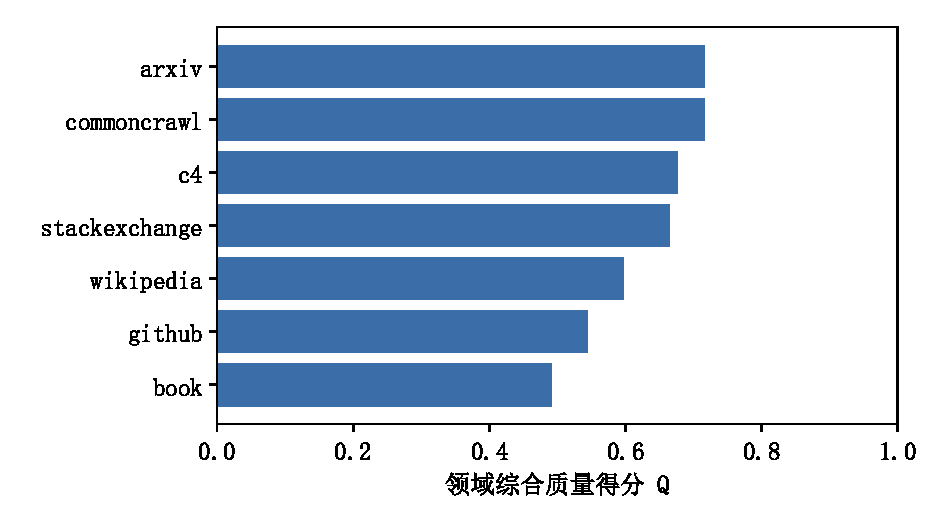
\includegraphics[width=0.92\textwidth]{figures/q1_fig02_domain_quality_scores.pdf}   % figure 4.2
          \caption{最终领域质量评分}
          \label{fig:qualitydomain}
        \end{figure}
        

        \subsubsection{A1 与扩展集的一致性}    % 4.3.2
        表4.3显示，arxiv 扩展集的平均质量比 A1 抽样低 0.00604，Cohen's $d=-0.0700$；github 的均值差仅 $-0.00126$，Cohen's $d=-0.0144$。arxiv 的 KS 检验因样本量大而达到统计显著，但效应量很小，不能据此声称抽样集与扩展集存在实质性质量差异。github 的分布差异也很小。扩展结果支持 A1 对这两个领域的均值代表性。
        
        \begin{table}[H]
        \centering
        \caption{A1 抽样与扩展集质量对照} % table 4.3
        \label{tab:extension}
        \begin{tabular}{lrrrrrr}
        \toprule
        领域 & $n_{A1}$ & $n_{ext}$ & $Q_{A1}$ & $Q_{ext}$ & 均值差 & Cohen's $d$ \\
        \midrule
        arxiv & 1,419 & 17,523 & 0.72287 & 0.71684 & $-0.00604$ & $-0.0700$ \\
        github & 10,000 & 203,752 & 0.54596 & 0.54470 & $-0.00126$ & $-0.0144$ \\
        \bottomrule
        \end{tabular}
        \end{table}
        
        \begin{figure}[H]
          \centering
          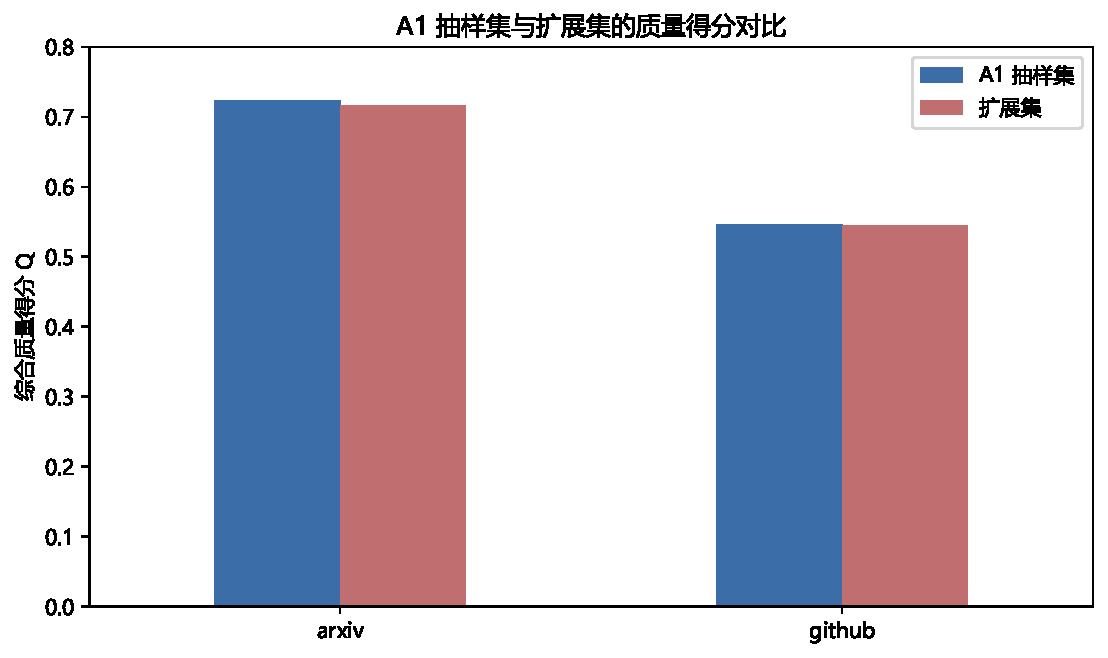
\includegraphics[width=0.80\textwidth]{figures/q1_fig03_extension_quality_comparison.pdf}  % figure 4.3
          \caption{A1 抽样与 A2/A3 扩展集平均质量比较}
          \label{fig:extension}
        \end{figure}


        \subsubsection{冲突结构与消解结果}  % 4.3.3
        全体 272,505 条记录的冲突率为 7.675\%。冲突贡献最高的指标为数字字符比例、词数、最高频三元字符比例、句数、最高频二元字符比例和广告信号，归一化贡献分别为 0.0617、0.0607、0.0569、0.0542、0.0538 和 0.0523。该结果说明冲突主要来自文本结构、长度和重复特征与模型型质量分之间的分歧，而非某个单一指标完全失效。
        
        \begin{figure}[H]
          \centering
          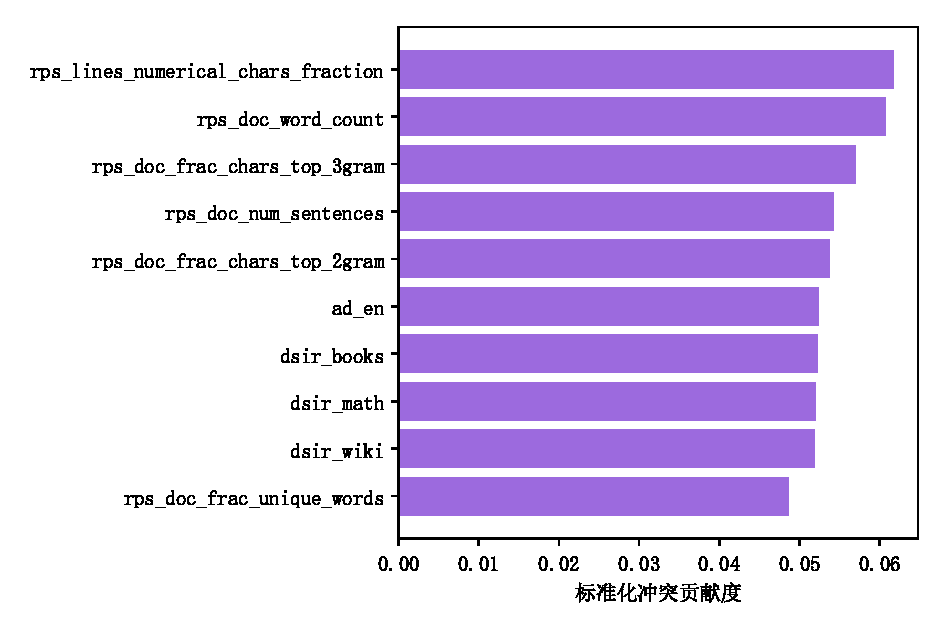
\includegraphics[width=0.93\textwidth]{figures/q1_fig04_conflict_metric_contributions.pdf}   % figure 4.4
          \caption{冲突记录中的主要指标贡献}
          \label{fig:conflictcontrib}
        \end{figure}
        
        Huber 聚合在冲突样本中降低大残差指标的有效权重，同时保留文本记录和其余指标。相比``检测冲突后删除样本''，该处理不会系统性排除包含公式、代码或特殊格式的高价值文本。置信度 $Conf_i$ 则将分歧程度和原始覆盖率显式保留下来，便于后续模型使用质量分时进行筛选或加权。


        \subsubsection{配比模型验证} % 4.3.4
        表8.5给出三组真实检验结果。1M 同规模检验取得 RMSE 0.28465、MAE 0.20269、$R^2=0.86473$，平均 Spearman 为 0.93396，说明二次 ILR 岭回归能够同时解释多数验证域的配比差异。
        
        60M 和 1B 的未校准 $R^2$ 为负，原因是模型规模改变了绝对 Loss 基准，而非配方排序失效。二者的平均 Spearman 仍为 0.92950 和 0.84253。使用检验标签做每个目标的一维仿射校准后，$R^2$ 分别达到 0.85178 和 0.81292；该结果只说明单调结构可通过尺度和平移校准，不视为独立预测性能。
        
        \begin{table}[H]
        \centering
        \caption{A6--A11 配比模型验证结果}  % table 4.4
        \label{tab:validation}
        \begin{threeparttable}
        \begin{tabular}{lrrrrrr}
        \toprule
        检验集 & RMSE & MAE & $R^2$ & 平均 Spearman & 校准 RMSE & 校准 $R^2$ \\
        \midrule
        1M & 0.28465 & 0.20269 & 0.86473 & 0.93396 & 0.27409 & 0.87458 \\
        60M & 1.59999 & 1.50659 & $-7.30804$ & 0.92950 & 0.21371 & 0.85178 \\
        1B & 2.70008 & 2.62433 & $-189.99642$ & 0.84253 & 0.08450 & 0.81292 \\
        \bottomrule
        \end{tabular}
        \begin{tablenotes}\small
        \item 注：60M、1B 的仿射校准使用相应检验标签，只用于描述跨规模单调迁移，不是独立预测。
        \end{tablenotes}
        \end{threeparttable}
        \end{table}
        
        \begin{figure}[H]   % figure 4.5
          \centering
          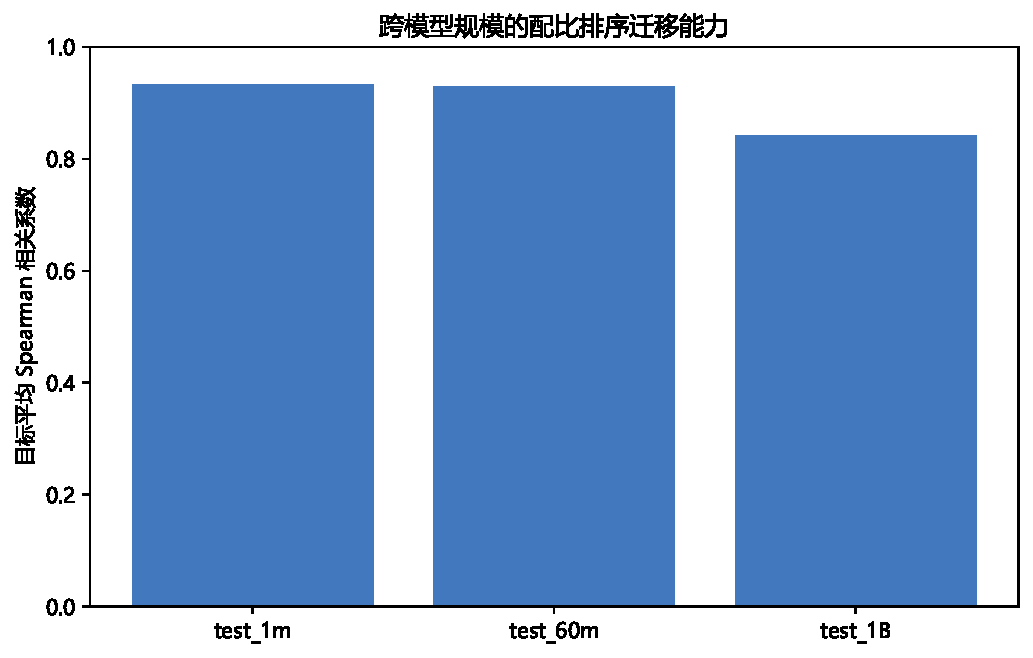
\includegraphics[width=0.78\textwidth]{figures/q1_fig05_mixture_validation_spearman.pdf}  % figure 4.5
          \caption{不同参数规模下的配方排序迁移}
          \label{fig:spearman}
        \end{figure}


        \subsubsection{领域主效应} % 4.3.5
        图4.5展示在 200 个训练配方附近计算的平均局部导数。dm\_mathematics、ubuntu\_irc、stackexchange 的平均导数分别为 $-7.216$、$-6.711$、$-6.515$，即增加 1 个百分点份额时，平均 Loss 的预测变化约为 $-0.0722$、$-0.0671$、$-0.0651$。enron\_emails、europarl 和 gutenberg\_pg\_19 的导数为正。由于不同参考配方下的导数标准差较大，这些数值应理解为样本分布上的平均局部关联。
        
        \begin{table}[H]
        \centering
        \caption{绝对值较大的领域局部边际效应}    % table 4.5    
        \label{tab:effects}
        \begin{tabular}{lrrl}
        \toprule
        领域 & $ME_k$ & 标准差 & 局部解释 \\
        \midrule
        dm\_mathematics & $-7.216$ & 7.897 & 增加份额通常降低 Loss \\
        ubuntu\_irc & $-6.711$ & 7.256 & 增加份额通常降低 Loss \\
        stackexchange & $-6.515$ & 9.119 & 增加份额通常降低 Loss \\
        enron\_emails & 5.354 & 14.464 & 增加份额通常提高 Loss \\
        freelaw & $-3.545$ & 8.092 & 增加份额通常降低 Loss \\
        arxiv & $-3.160$ & 6.573 & 增加份额通常降低 Loss \\
        github & $-3.139$ & 7.928 & 增加份额通常降低 Loss \\
        europarl & 2.252 & 8.100 & 增加份额通常提高 Loss \\
        \bottomrule
        \end{tabular}
        \end{table}
        
        \begin{figure}[H]
          \centering
          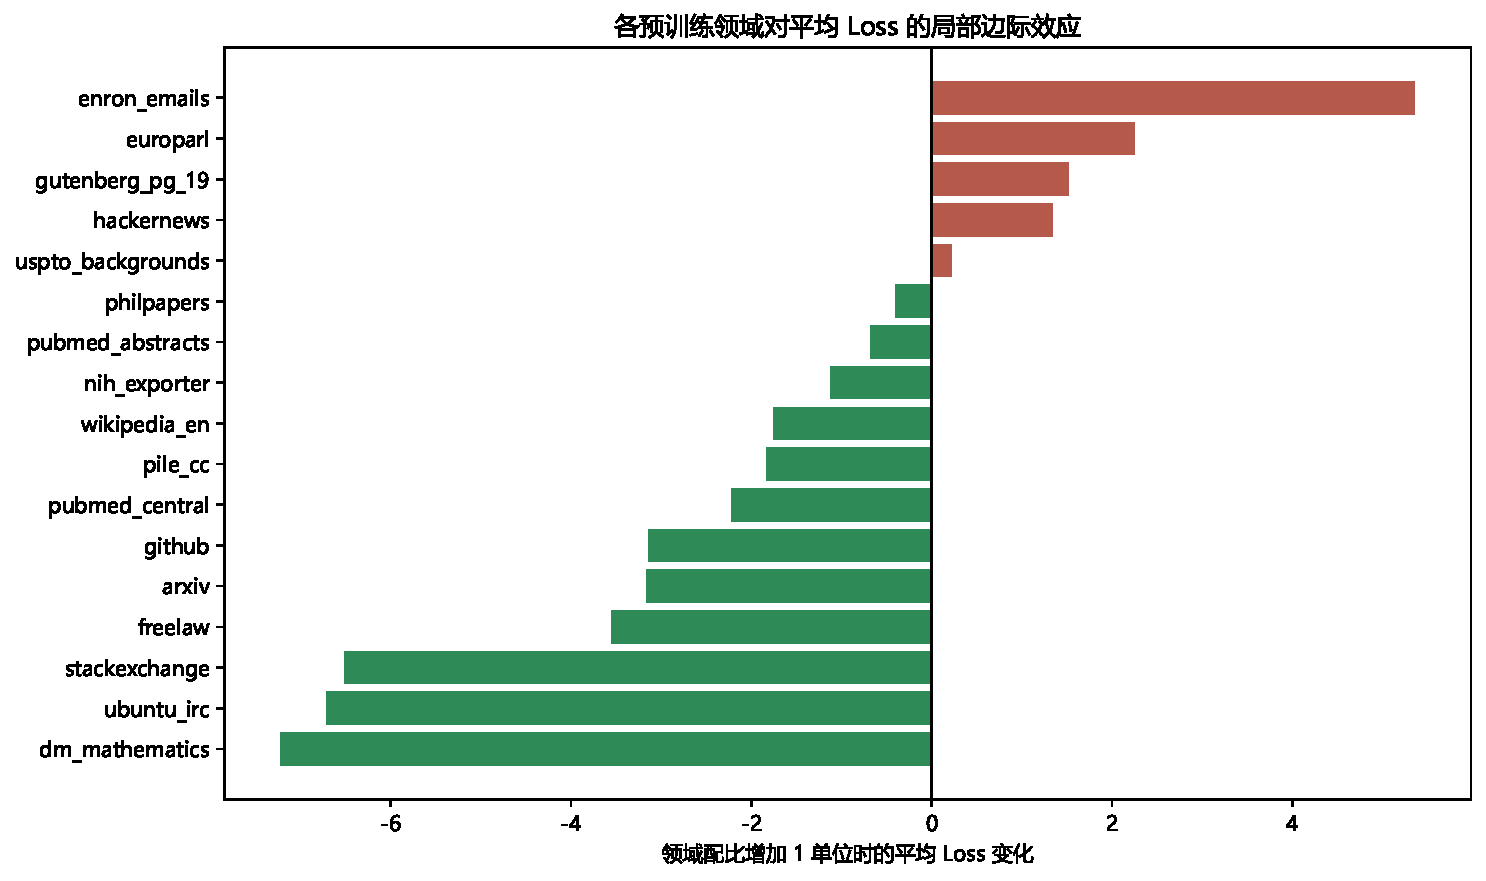
\includegraphics[width=0.96\textwidth]{figures/q1_fig06_mixture_domain_effects.pdf}   % figure 4.6
          \caption{17 个训练领域对平均 Loss 的局部边际效应}
          \label{fig:maineffect}
        \end{figure}


        \subsubsection{领域组合效应} % 4.3.6
        二阶差分绝对值最大的组合多涉及样本中较稀疏的 philpapers、nih\_exporter 和 enron\_emails。例如 philpapers--enron\_emails 的 $INT=87.85$，表示组合效果弱于主效应可加预期；enron\_emails--europarl 的 $INT=-18.33$，表现为局部协同。由于二阶效应对配方位置和伪计数更敏感，本文只把其作为筛选需要进一步实验的领域组合，不把数值直接解释为稳定因果效应。
        
        \begin{table}[H]
        \centering
        \caption{绝对值最大的领域组合效应}  % table 4.6
        \label{tab:interactions}
        \begin{tabular}{llrr}
        \toprule
        领域 1 & 领域 2 & $INT_{jk}$ & 类型 \\
        \midrule
        philpapers & enron\_emails & 87.85 & 拮抗 \\
        nih\_exporter & philpapers & 59.38 & 拮抗 \\
        nih\_exporter & enron\_emails & 51.52 & 拮抗 \\
        enron\_emails & hackernews & 44.71 & 拮抗 \\
        philpapers & europarl & 27.07 & 拮抗 \\
        enron\_emails & europarl & $-18.33$ & 协同 \\
        enron\_emails & gutenberg\_pg\_19 & 17.38 & 拮抗 \\
        nih\_exporter & europarl & 13.44 & 拮抗 \\
        \bottomrule
        \end{tabular}
        \end{table}


        \subsubsection{质量映射覆盖与不可辨识性}    % 4.3 7
        A16 的直接或近直接映射只覆盖 6 个配方域。训练配方中，已映射领域份额的平均值为 0.5646，即平均有 56.46\% 的语料份额能够对应到已有质量评分，1M/60M 检验为 0.5690，1B 为 0.6224；不同配方的覆盖质量从接近 0 到 1 不等。训练集的 $Q_{mix}$ 部分识别区间平均宽度为 0.0983，1M/60M 为 0.0973，1B 为 0.0852。该宽度表明，对未映射 11 域强行填入单一质量分会制造不可忽略的模型确定性。本文因此保留上下界，并将 $Q_{mix}^{mid}$ 只作为敏感性描述量。
        
        \begin{table}[H]
        \centering
        \caption{配方质量映射覆盖情况}    % table 4.7
        \label{tab:mapping}
        \begin{tabular}{lrrrr}
        \toprule
        数据集 & 样本量 & 已映射领域份额均值 & 已映射领域份额范围 & 平均区间宽度 \\
        \midrule
        训练 1M & 512 & 0.5646 & 0.000--1.000 & 0.0983 \\
        检验 1M & 256 & 0.5690 & 0.001--1.000 & 0.0973 \\
        检验 60M & 256 & 0.5690 & 0.001--1.000 & 0.0973 \\
        检验 1B & 64 & 0.6224 & 0.138--0.888 & 0.0852 \\
        外推 10B/70B & 各 63 & 0.5435 & 0.003--1.000 & 0.1030 \\
        \bottomrule
        \end{tabular}
        \end{table}


        \subsubsection{外推稳定性}   % 4.3.8
        A12--A15 上的未校准绝对误差很大，符合模型规模改变 Loss 基准的预期。10B 和 70B 的配方排序平均 Spearman 分别为 0.60949 和 0.52874；使用外推标签做仿射校准后 $R^2$ 分别为 0.57882 和 0.45793。该结果说明效应排序具有中等稳定性，但明显弱于真实 60M/1B 检验。由于外推配比为训练子集、Loss 也来自外推，本文不把它作为真实大模型实验验证。
        
        \begin{table}[H]
        \centering
        \caption{A12--A15 外推稳定性结果}  % table 4.8
        \label{tab:extrapolation}
        \begin{tabular}{lrrrr}
        \toprule
        数据集 & 未校准 RMSE & 平均 Spearman & 校准 RMSE & 校准 $R^2$ \\
        \midrule
        10B 外推 & 3.62349 & 0.60949 & 0.17124 & 0.57882 \\
        70B 外推 & 4.01115 & 0.52874 & 0.16192 & 0.45793 \\
        \bottomrule
        \end{tabular}
        \end{table}


        \subsubsection{小结}  % 4.3.9
        本节完成了问题一的质量评价、冲突消解和领域配比建模。基于 272,505 条记录构建的 Huber 综合质量分能够统一 22 个异质指标。arxiv 与 commoncrawl 的领域质量最高，github 与 book 较低；book 的样本量和冲突结构使其不确定性更大。总体冲突率为 7.675\%。冲突主要与数字比例、文本长度和重复统计有关。Huber 估计能够在不删除文本的情况下抑制离群指标。arxiv、github 的扩展集与 A1 抽样集平均质量差异很小，Cohen's $d$ 的绝对值均小于 0.08，支持 A1 的均值代表性ILR 二次岭回归在 1M 检验集上达到 $R^2=0.86473$，跨到 60M 和 1B 后配方排序相关仍为 0.92950 和 0.84253。配比规律主要以相对排序形式迁移，绝对 Loss 需要规模校准在观测配方邻域内，dm\_mathematics、ubuntu\_irc、stackexchange 的平均边际效应最有利；enron\_emails 的平均效应不利。该结论仅适用于局部调整。A16 的映射覆盖不足以识别独立质量系数。部分识别区间比主观补值更诚实，也为问题二引入质量因素提供了不确定性边界。


\section{问题二}   % 5
    \subsection{问题分析}
    质量评分、领域配比和模型规模来自不同的实验体系，不能将全部 Loss 记录直接拼接后回归。一方面，问题一的质量映射只覆盖部分训练领域，其余领域只能给出条件区间；另一方面，质量代表值本身是配比的线性组合，如果同时将质量代表值和全部份额作为自由解释变量，难以识别独立质量作用。因此，本问沿用问题一的质量与配比结果，将“改变配方”和“固定配方后额外改善质量”分开建模。

    规模信息由 B1 的训练轨迹提供，质量响应主要由 B6 中固定参数量、数据量后改变质量的记录提供。B6 的半合成性质以及不同来源的评价口径差异，决定了质量响应系数 $\gamma$ 只能作为条件迁移参数，不能直接解释为真实训练中的统一规律。B7 还包含与 B6 重复的记录，必须先去重再检验；插值和估算数据只用于一致性分析。

    参考计算最优训练的双幂律框架\textsuperscript{\cite{hoffmann2022chinchilla}}以及数据配比与训练规模相衔接的研究思路\textsuperscript{\cite{ye2025mixing}}，本文采用“经典标度律参数估计、质量响应系数估计、配比相对响应修正”的分阶段建模方法。以双幂律刻画参数量和训练数据量的影响，用当前配方与参考配方的平均预测 Loss 之比表示配比响应，再通过正值修正因子将额外质量改善接入模型。模型建立后，利用留出检验与跨来源比较确定适用范围，并推导边际收益、质量与参数的等效替代条件，以及单纯形内的领域局部交互关系。

    \subsection{模型建立}
        \subsubsection{数据整理与问题一结果衔接}  % 5.2.1
        以验证集交叉熵损失 $L$ 为评价指标，数值越小表示预测性能越好。为统一数量级，记
        \begin{equation}
         n=\frac{N}{10^9},\qquad d=\frac{D}{10^{11}},\qquad
         \bm p=(p_1,\ldots,p_{17})^\mathsf T,\quad
         p_j\geq0,\quad\sum_{j=1}^{17}p_j=1.
         \label{eq:p2_units}
        \end{equation}
        其中，$n=7,d=3$ 分别对应 70 亿参数与 3000 亿 tokens。对附件中的配比先归一化，使各领域份额之和等于 1，再调用问题一的预测模型。
        
        问题一的接口包括领域质量、512 个训练配方及其已拟合的配比模型。这里的一个配方是由 17 个领域份额组成的向量，512 个配方对应 512 种训练语料混合方案。取这些配方的算术均值为参考配比 $\bm p_0$。质量数据与配方数据的领域分类并不完全对应，仅有 6 个配方域能够直接或近似映射，其余 11 个域沿用问题一的敏感性代表值，即全局加权质量均值 $q_G$，构造可计算的常规质量基准。设可映射领域集合为 $M$，定义配方的常规质量为
        \begin{equation}
         \bar q_j=\begin{cases}q_j,&j\in M,\\q_G,&j\notin M,\end{cases}
         \qquad \bar Q(\bm p)=\sum_{j=1}^{17}p_j\bar q_j,
         \qquad Q_0=\bar Q(\bm p_0)=0.610914.
         \label{eq:p2_quality}
        \end{equation}
        $Q_0$ 只用于归一化，不代表对 B1 训练语料质量的实际测量。该代表值并非新增的质量观测，也不取代问题一的部分识别区间；在敏感性分析中，将其取值范围设为已观测领域质量的最小值至最大值，得到条件性的配方质量区间。
        
        Pythia 提供在受控训练设置下的多规模模型及中间检查点，为分析训练规模与训练进程提供了实验背景\textsuperscript{\cite{biderman2023pythia}}。本研究的具体观测及其证据性质以赛事附件和数据说明为准。规模参数主要由 B1 的 1176 个训练检查点估计，覆盖 8 个参数规模；质量响应由 B6 的 360 条半合成记录估计。B7 的 450 条记录中有 360 条与 B6 完全重合，故只保留其余 90 条用于新质量水平验证。B3 为基于 B1 生成的插值数据，B10 为估算损失，二者均不作为新增真实实验。B2、B4、B5 用于跨来源迁移检验，B8 用于质量方向的一致性审查。对 B9 排除 4 条规模缺失或非正的记录，其余 128 条仅用于大模型情景预测。
    
        \subsubsection{经典标度律}  % 5.2.2
        借鉴 Hoffmann 等提出的参数量与训练数据量双幂律形式\textsuperscript{\cite{hoffmann2022chinchilla}}，以参数受限和数据受限造成的超额损失构造规模基准，并使用附件 B 重新估计系数和指数：
        \begin{equation}
         L_0(n,d)=E+A n^{-\alpha}+B d^{-\beta},\qquad
         X=A n^{-\alpha},\quad Y=B d^{-\beta}.
         \label{eq:p2_baseline}
        \end{equation}
        其中 $E\geq0$ 为该模型下的渐近损失水平，$A,B>0$ 决定两类超额损失的幅度，$\alpha,\beta>0$ 表示规模增长的衰减速度。因而 $X$ 和 $Y$ 均随相应资源增加而减小。
        
        \subsubsection{质量与配比修正因子}  % 5.2.3
        在 RegMix 的配比性能代理预测思路基础上\textsuperscript{\cite{liu2025regmix}}，复用问题一采用 ILR 坐标与岭正则化构建的二次回归模型\textsuperscript{\cite{egozcue2003ilr,hoerl1970ridge}}，将 13 个验证域的预测损失取算术平均，记为 $f_A(\bm p)$。为避免直接叠加不同评价口径下的绝对损失，使用相对响应
        \begin{equation}
         f_A(\bm p)=\frac1{13}\sum_{r=1}^{13}\widehat L_{A,r}(\bm p),
         \qquad h(\bm p)=\log\frac{f_A(\bm p)}{f_A(\bm p_0)}.
         \label{eq:p2_mix}
        \end{equation}
        于是 $h(\bm p_0)=0$，$h(\bm p)<0$ 表示该配方在问题一模型中优于参考配方。该定义要求所用配方的预测损失为正；本文在已计算的配方及参考点邻域内使用该响应。
        
        已有研究通过质量因子修正标度律的数据项\textsuperscript{\cite{subramanyam2026quality}}，为显式引入质量提供了参考；其质量定义与本文的综合评分并不等同。本文进一步假设，固定配比后的额外质量改善按比例减少参数项与数据项之和所构成的超额损失。下式中的指数质量修正、相对配比响应及其组合方式均为本文的建模设定，并通过对照检验与敏感性分析考察适用性。将两种响应结合，得到
        \begin{equation}
         \begin{aligned}
         G(Q,\bm p)&=\exp\!\left\{\gamma\kappa[\bar Q(\bm p)-Q]+\lambda_p h(\bm p)\right\},\\
         L(n,d,Q,\bm p)&=E+\left(A n^{-\alpha}+B d^{-\beta}\right)G(Q,\bm p).
         \end{aligned}
         \label{eq:p2_general}
        \end{equation}
        其中 $\gamma\geq0$ 为质量响应系数，$\kappa$ 表示附件 A 与 B 的质量尺度换算系数，$\lambda_p$ 表示配比效应的迁移强度。主情景设 $\kappa=\lambda_p=1$，并另行讨论其变化。现有附件不能唯一识别这两个迁移系数，故该设定属于模型假设。
        
        式\eqref{eq:p2_general}具有三个便于解释的性质。第一，在参考条件 $\bm p=\bm p_0,Q=Q_0$ 下，$G=1$，模型退化为式\eqref{eq:p2_baseline}。第二，改变配方且使用其常规质量，即 $Q=\bar Q(\bm p)$ 时，质量偏离项为零，已有的配方差异仅通过 $h(\bm p)$ 起作用，从而避免重复计入质量贡献。第三，固定规模与配比，将质量提高 $\Delta Q$ 后，有
        \begin{equation}
         \frac{L(n,d,Q+\Delta Q,\bm p)-E}{L(n,d,Q,\bm p)-E}
         =\exp(-\gamma\kappa\Delta Q),\qquad Q+\Delta Q\leq1.
         \label{eq:p2_qchange}
        \end{equation}
        这表示质量改善作用于可减少的损失部分，而不改变模型设定的渐近水平 $E$。
        
        \subsubsection{分阶段稳健参数估计}  % 5.2.4
        第一阶段，在 B1 上估计 $\bm\theta=(E,A,B,\alpha,\beta)$。由于同一规模下的后期检查点较密集，先将全局 $\log d$ 范围划为 8 个等宽区间，再使各规模、各非空区间获得均衡权重。若规模 $g$ 有 $K_g$ 个非空区间，区间 $(g,b)$ 内有 $m_{gb}$ 条记录，则原始权重为 $1/(K_gm_{gb})$，归一化后记为 $\omega_i$。令 $e_i(\bm\theta)=L_0(n_i,d_i)-L_i$，求解
        \begin{equation}
         \widehat{\bm\theta}=\arg\min_{\bm\theta}
         \sum_i\delta^2\left[\sqrt{1+\frac{\omega_i e_i(\bm\theta)^2}{\delta^2}}-1\right],
         \qquad \delta=0.1.
         \label{eq:p2_fit}
        \end{equation}
        该目标采用 Soft-L1 平滑鲁棒损失，在小残差附近接近平方损失，在大残差处减小异常值的影响。数值实现采用 SciPy 的 \texttt{least\_squares}，设置 \texttt{loss='soft\_l1'}，并通过多初值有界非线性最小二乘求解\textsuperscript{\cite{virtanen2020scipy}}。均衡权重、分阶段拟合及参数边界均为针对附件结构所作的实现选择。限制 $0\leq E<\min_iL_i$、$10^{-8}\leq A,B\leq30$、$0.005\leq\alpha,\beta\leq2$。
        
        第二阶段，固定第一阶段的指数，为 B6 设置独立的基线系数：
        \begin{equation}
         L_{6,i}=E_6+\left(A_6n_i^{-\widehat\alpha}+B_6d_i^{-\widehat\beta}\right)
         \exp\!\left\{\gamma(Q_0-Q_i)\right\}+\varepsilon_i.
         \label{eq:p2_fit_quality}
        \end{equation}
        仍采用稳健最小二乘，取 $\delta=0.05$，联合估计 $E_6,A_6,B_6,\gamma$。主模型只接收质量响应 $\gamma$，其规模基线仍采用 B1 的参数，从而允许 B1 与 B6 存在绝对损失差异。
    
        \subsubsection{验证设计与不确定性估计}  % 5.2.5
        在 B1 上分别实施按参数规模留出和按训练阶段留出。前者每次留出一个规模的完整训练轨迹，合并八次留出预测评价泛化误差；后者对各规模按数据量排序，以前 70\% 检查点拟合、后 30\% 检查点检验。B6 按完整 $(N,D)$ 组进行五折交叉验证，同组质量水平进入同一折，比较无质量项、共享规模指数和自由规模指数三类模型。
        
        预测误差采用
        \begin{equation}
         \operatorname{RMSE}=\sqrt{\frac1m\sum_{i=1}^{m}(L_i-\widehat L_i)^2}.
         \label{eq:p2_rmse}
        \end{equation}
        配比迁移则对 13 个验证域平均 Loss 的排序计算 Spearman 相关系数。该指标与问题一“先对各验证域计算相关系数再求平均”的指标不同，分别报告，避免混用。
        
        借鉴 Bootstrap 重抽样估计不确定性的思想\textsuperscript{\cite{efron1979bootstrap}}，考虑同一轨迹或实验组内记录的相关性，本文对 B1 按完整规模轨迹、对 B6 按完整 $(N,D)$ 组进行 200 次重采样，每次重新估计两阶段参数，并以 2.5\% 与 97.5\% 分位数构造条件 95\% 区间。质量量尺 $\kappa$ 和配比迁移强度 $\lambda_p$ 另行进行敏感性分析，不将这些结构假设的不确定性混入抽样区间。
    
        \subsubsection{边际收益与单位成本条件}  % 5.2.6
        令 $\eta=\gamma\kappa$，将增加单位资源带来的损失减少量定义为边际收益。固定其他变量，由式\eqref{eq:p2_general}可得
        \begin{equation}
         U_n=-\frac{\partial L}{\partial n}=\frac{\alpha XG}{n},\qquad
         U_d=-\frac{\partial L}{\partial d}=\frac{\beta YG}{d},\qquad
         U_Q=-\frac{\partial L}{\partial Q}=\eta(X+Y)G.
         \label{eq:p2_marginal}
        \end{equation}
        $U_n$ 对应每增加十亿参数的局部收益，$U_d$ 对应每增加一千亿 tokens 的局部收益，两者不能忽略单位直接比较。对超额损失 $F=L-E$，进一步定义无量纲的改进弹性：
        \begin{equation}
         \epsilon_n^F=\frac{\alpha X}{X+Y},\qquad
         \epsilon_d^F=\frac{\beta Y}{X+Y},\qquad
         \epsilon_Q^F=\eta Q.
         \label{eq:p2_elasticity}
        \end{equation}
        
        
        三种资源方向上的二阶导数均非负，参数量与数据量方向严格为正，表明模型具有边际收益递减特征。参数量与质量的混合导数为 $\eta\alpha XG/n\geq0$，意味着在本模型中，质量改善会降低继续扩容的边际降损收益，二者表现为局部替代。
        
        设增加十亿参数的边际成本为 $c_n>0$，提高一个质量单位的边际成本为 $c_Q>0$。比较 $U_n/c_n$ 与 $U_Q/c_Q$，得到优先改善质量的条件
        \begin{equation}
         \frac{c_Q}{c_n}<\frac{\eta n(X+Y)}{\alpha X}.
         \label{eq:p2_cost}
        \end{equation}
        附件未提供与该场景对应的真实货币成本，故本问给出临界成本比，不据此认定某一方案必然更便宜。若固定总训练算力 $C=6ND$，扩容会同时减少可用训练数据量，此时沿算力约束的收益变为 $G(\alpha X-\beta Y)/n$，只有 $\alpha X>\beta Y$ 时继续增加参数才有利。
    
        \subsubsection{质量提高与参数扩容的等效条件}  % 5.2.7
        固定数据量与配比，比较两种达到同样损失的方案：一是保持参数量 $n$，将质量从 $Q$ 提高至 $Q+\Delta Q$；二是保持原质量，将参数量提高至 $n_{\mathrm{eq}}$。令 $t=\exp(-\eta\Delta Q)$，消去相同的 $E$ 和原修正因子后，有
        \begin{equation}
         A n_{\mathrm{eq}}^{-\alpha}+Y=t(X+Y),\qquad
         \frac{n_{\mathrm{eq}}}{n}=\left[\frac{t(X+Y)-Y}{X}\right]^{-1/\alpha}.
         \label{eq:p2_equiv}
        \end{equation}
        有限等效扩容解要求 $t(X+Y)>Y$。当 $\eta>0$ 时，这一条件等价于
        \begin{equation}
         0<\Delta Q<\frac1\eta\log\left(1+\frac XY\right),\qquad Q+\Delta Q\leq1.
         \label{eq:p2_equiv_bound}
        \end{equation}
        当等式边界成立时，需要的参数量趋于无穷；超过该边界后，质量提升带来的目标损失已低于固定数据量下仅靠扩容所能达到的极限。因此，质量改善并不总能用有限参数扩容来等价替代。
    
        \subsubsection{领域边际作用与局部交互}  % 5.2.8
        由于配比之和固定，提高某个领域份额必须相应减少其他份额。本文固定参数量与数据量，在参考配比 $\bm p_0$ 附近分析，并沿 $Q=\bar Q(\bm p)$ 的常规质量路径改变配方。对单一领域 $j$，取 $v_{j,j}=1$，其余分量为 $v_{j,l}=-p_{0,l}/(1-p_{0,j})$，即其余领域按比例让出份额。计算方向导数 $D_{v_j}L$，负值表示这一局部调整能够降低平均损失。
        
        对领域 $j,k$ 的交互，使用其余 15 个领域组成的共同供给池。令 $\bm e_j$ 为第 $j$ 个单位向量，定义
        \begin{equation}
         u_l=\begin{cases}0,&l\in\{j,k\},\\
         \dfrac{p_{0,l}}{1-p_{0,j}-p_{0,k}},&l\notin\{j,k\},\end{cases}
         \qquad \bm v_j=\bm e_j-\bm u,\quad \bm v_k=\bm e_k-\bm u.
         \label{eq:p2_pool}
        \end{equation}
        将两个方向固定在参考点，记 $\ell(\bm p)=L(n,d,\bar Q(\bm p),\bm p)$，以步长 $\varepsilon_p=10^{-4}$ 的四角中心差分计算混合导数：
        \begin{equation}
         \begin{aligned}
         I_{jk}\approx\frac1{4\varepsilon_p^2}\big[&\ell(\bm p_0+\varepsilon_p\bm v_j+\varepsilon_p\bm v_k)
         -\ell(\bm p_0+\varepsilon_p\bm v_j-\varepsilon_p\bm v_k)\\
         &-\ell(\bm p_0-\varepsilon_p\bm v_j+\varepsilon_p\bm v_k)
         +\ell(\bm p_0-\varepsilon_p\bm v_j-\varepsilon_p\bm v_k)\big].
         \end{aligned}
         \label{eq:p2_interaction}
        \end{equation}
        $I_{jk}<0$ 表示增加一个领域会使另一个方向的边际降损作用增强，称为该路径下的局部互补；$I_{jk}>0$ 表示边际降损作用减弱，称为局部替代。

    \subsection{建模结果}
        \subsubsection{参数估计与规模拟合}  % 5.3.1
        表\ref{tab:p2_parameters}给出两阶段主参数及条件 Bootstrap 区间。所有估计均未落在数值求解边界上。区间只反映给定模型与数据生成方式下的抽样变化，不包含质量量尺和跨来源迁移假设的不确定性。

        \begin{table}[H]
         \centering
         \caption{广义标度律的参数估计}
         \label{tab:p2_parameters}
         \begin{tabular}{ccc}
          \toprule
          参数 & 点估计 & 条件 Bootstrap 95\% 区间 \\
          \midrule
          $E$ & 1.689482 & [1.688891, 1.690181] \\
          $A$ & 0.354064 & [0.353349, 0.354692] \\
          $B$ & 0.342016 & [0.341785, 0.342208] \\
          $\alpha$ & 0.339921 & [0.339433, 0.340627] \\
          $\beta$ & 0.279796 & [0.279714, 0.279893] \\
          $\gamma$ & 0.410160 & [0.389385, 0.433103] \\
          \bottomrule
         \end{tabular}
        \end{table}
        
        图\ref{fig:p2_scaling}展示了 B1 检查点与拟合曲线。图中散点为附件值，曲线为模型预测结果。随训练数据量增大，各参数规模下的损失逐渐下降，且下降幅度逐步减小；相同数据量下，较大模型通常对应较低损失。全量拟合的 RMSE 为 $1.522\times10^{-4}$，说明附件曲线与所设函数形式高度一致。
        
        \begin{figure}[H]
         \centering
         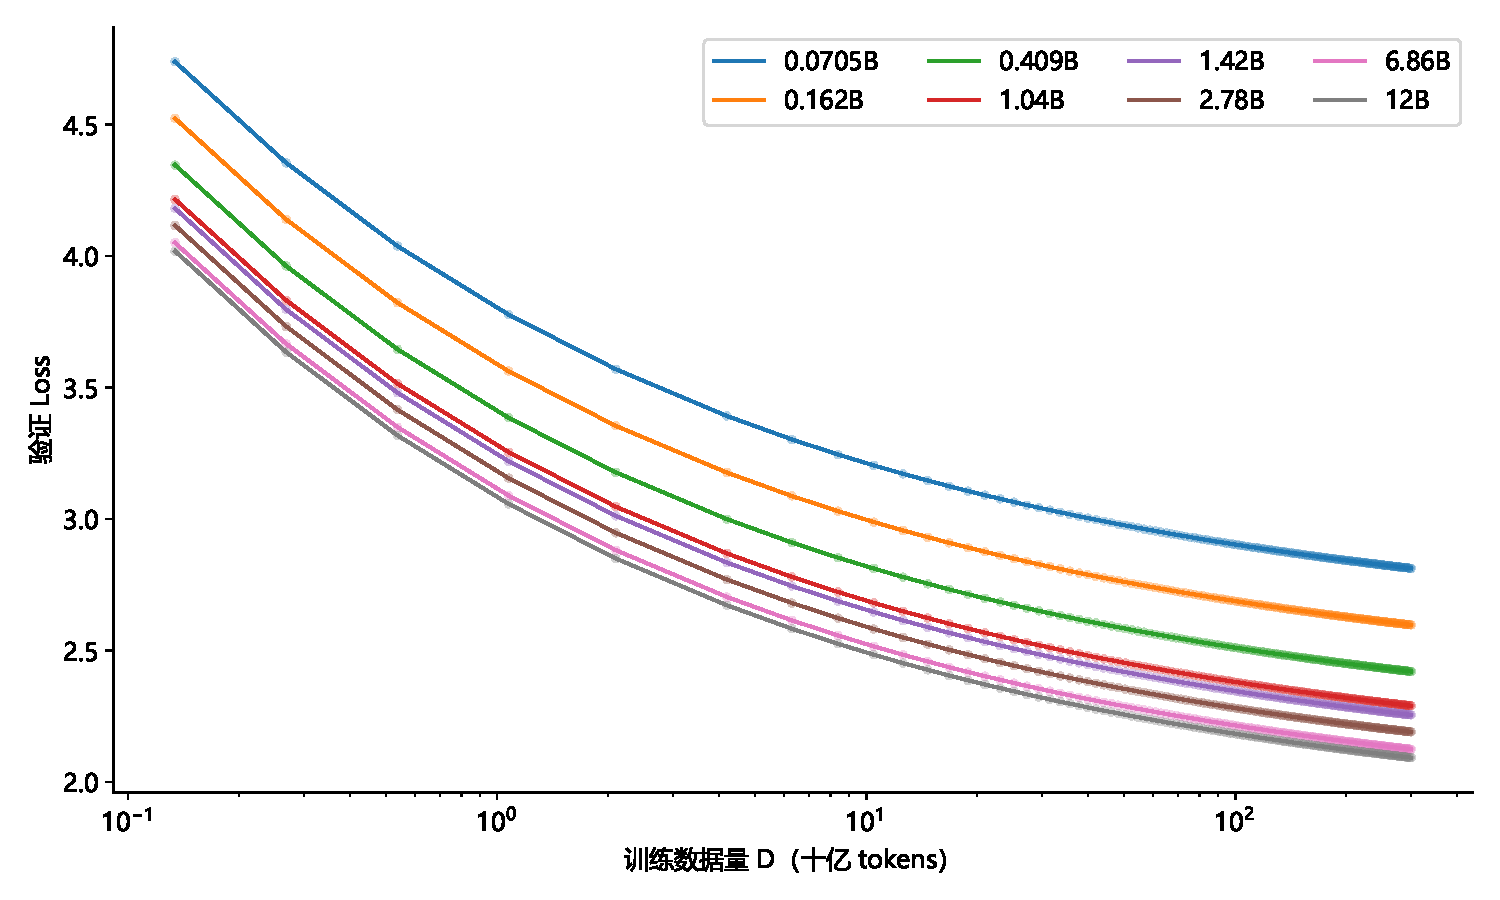
\includegraphics[width=\linewidth]{figures/q2_fig01_scaling_fit.pdf}
         \caption{B1 的训练检查点与经典标度律拟合}
         \label{fig:p2_scaling}
        \end{figure}

        \subsubsection{分层验证与质量项贡献}  % 5.3.2
        无质量项模型的平均 RMSE 为 0.129993，加入质量项后降至 0.054591，约降低 58.0\%；允许 B6 单独估计规模指数时进一步降至 0.052462。因此，质量项在该半合成数据内有效，但共享规模指数并非唯一可能的设定。上述对照分别检验质量项的贡献与规模指数共享假设。
        
        \begin{table}[H]
         \centering
         \caption{B6 质量项消融与共享指数检验}
         \label{tab:p2_quality_ablation}
         \begin{tabular}{lc}
          \toprule
          模型 & 五折分组验证平均 RMSE \\
          \midrule
          无质量项模型 & 0.129993 \\
          共享 B1 指数的质量模型 & 0.054591 \\
          自由指数质量模型 & 0.052462 \\
          \bottomrule
         \end{tabular}
        \end{table}
        
        主要检验结果见表\ref{tab:p2_validation}。B1 两类留出的误差均较小，但 B2 的直接迁移误差显著增大，B4 与 B5 也保留明显误差，说明仅使用同一组规模参数不足以消除来源间的评价口径差异。尤其是 B1 的误差已接近附件的数值舍入精度，不能据此推断任意真实训练实验都会达到同样精度。
        
        \begin{table}[H]
         \centering
         \caption{分层检验结果及其证据性质}
         \label{tab:p2_validation}
         \begin{tabularx}{\linewidth}{@{}l r >{\raggedright\arraybackslash}X@{}}
          \toprule
          检验方式 & RMSE & 解释范围 \\
          \midrule
          B1 留出参数规模 & 0.000181 & 同来源的未参与拟合规模 \\
          B1 留出后期检查点 & 0.000143 & 同来源的后期训练阶段 \\
          B2 直接迁移 & 1.243161 & 半合成数据，迁移误差较大 \\
          B3 轨迹比较 & 0.003799 & B1 派生插值的一致性 \\
          B4 跨模型族迁移 & 0.292703 & 跨来源记录，损失口径未统一 \\
          B5 文献数据迁移 & 0.197572 & 公开结果的有限迁移检验 \\
          B7 去重新增点 & 0.043803 & 90 个半合成的新质量水平 \\
          B8 直接预测 & 1.350759 & 质量方向冲突检验 \\
          B10 估算值比较 & 0.001049 & 估算机制的一致性 \\
          \bottomrule
         \end{tabularx}
        \end{table}
        
        \subsubsection{质量方向冲突}  % 5.3.3
        进一步固定 $(N,D)$ 检查质量变化方向。B6 的 45 个组中，质量与损失的线性趋势斜率均为负；B8 的 150 个组则全部为正。图\ref{fig:p2_conflict}将各组损失减去组内均值，以突出这种方向差异。图中每条折线对应固定的 $(N,D)$ 组，纵轴为组内中心化损失。因此，B8 与主模型的单调质量假设冲突，不纳入质量收益估计，也不通过反转质量分数来消除冲突。该结果限定了主模型的适用范围：质量改善结论以 B6 的质量定义和变化机制能够迁移为前提。
        
        \begin{figure}[H]
         \centering
         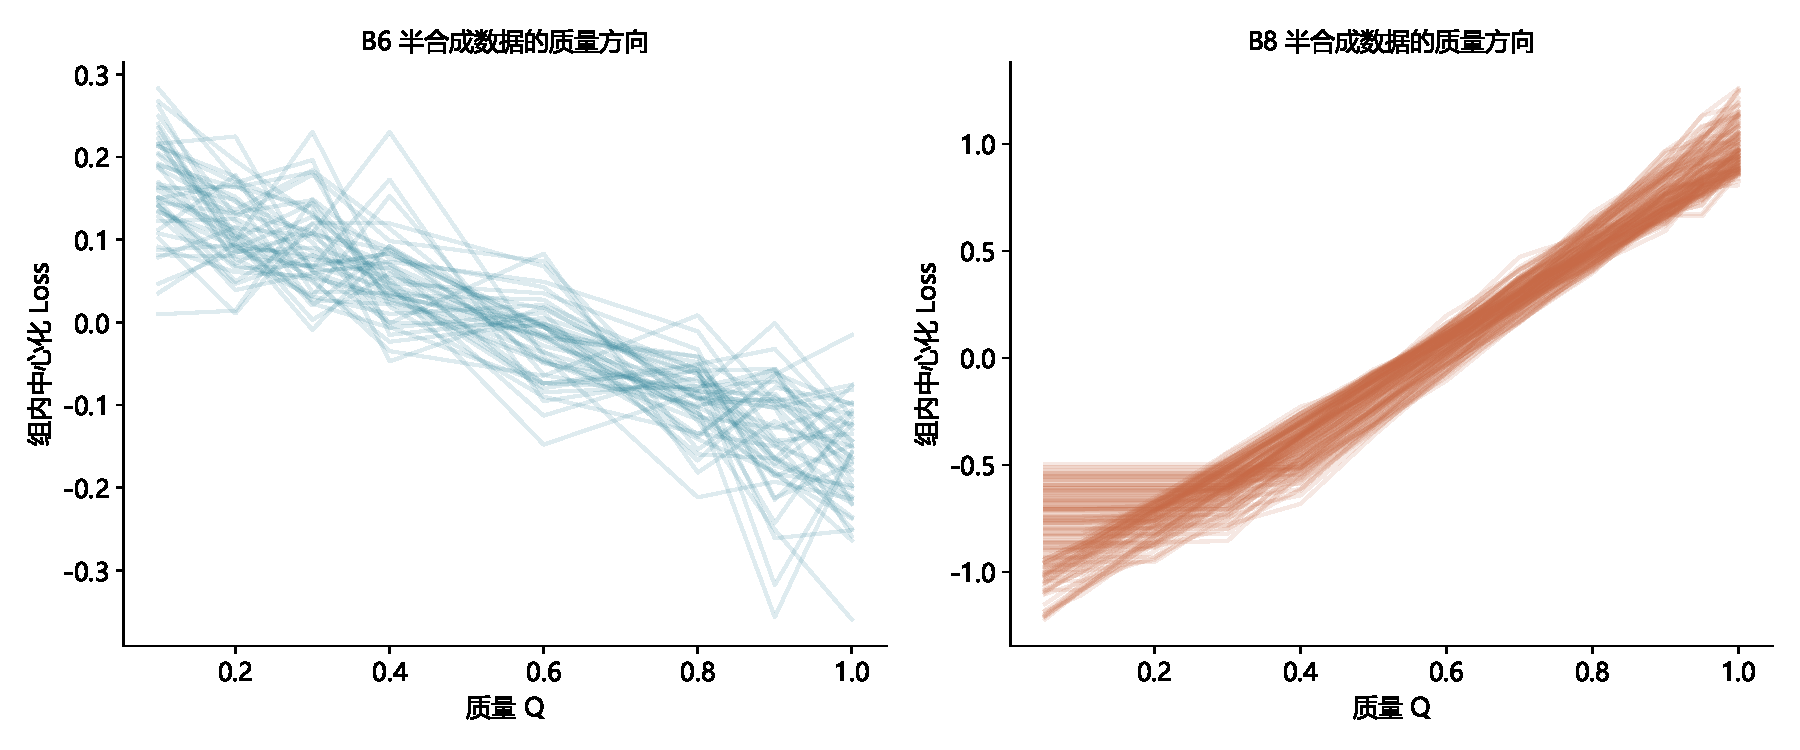
\includegraphics[width=\linewidth]{figures/q2_fig02_quality_direction_conflict.pdf}
         \caption{B6 与 B8 的质量方向比较}
         \label{fig:p2_conflict}
        \end{figure}
        
        \subsubsection{边际收益与成本比较}  % 5.3.4
        在 $n=7, d=3, \bm p=\bm p_0, Q=Q_0$ 的主情景下，超额 Loss 关于参数量、数据量和质量的改进弹性分别为 0.1430、0.1621 和 0.2506。例如，参数量局部增加 1\%，对应超额损失约减少 0.143\%。由于 $Q$ 是有界综合评分，质量改善还需结合式\eqref{eq:p2_qchange}中的绝对增量解释。
        
        在相同参考条件下，每增加 1B 参数的边际降损收益约为 0.008874，每增加 1B tokens 的收益约为 0.000235，提高一个质量单位的收益约为 0.178108。以上均为局部导数，质量提高 0.1 的有限变化仍应采用式\eqref{eq:p2_qchange}计算。
        
        式\eqref{eq:p2_cost}给出的临界成本比为 20.0718。由于缺少清洗筛选成本和对应训练成本，现有数据尚不能用于估计具体的货币节省金额。该条件为后续在成本约束下比较扩容、增加数据和改善质量提供接口。
        
        \subsubsection{质量提升的等效扩容结果}  % 5.3.5
        取 $N=7$B、$D=300$B、$\bm p=\bm p_0$，质量由 0.610914 提高至 0.710914。主情景的计算结果为
        \begin{equation}
         \begin{aligned}
         L_{\mathrm{before}}&=2.123722,\qquad L_{\mathrm{after}}=2.106271,\\
         N_{\mathrm{eq}}&=9.404464\text{B},\qquad N_{\mathrm{eq}}/N=1.343495.
         \end{aligned}
         \label{eq:p2_example}
        \end{equation}
        即质量提高 0.1 所带来的预测改进，约等价于增加 34.35\% 的参数。扩容倍数的条件 Bootstrap 95\% 区间为 $[1.322870,1.366724]$。该例是模型计算结果，并非真实对照实验；300B tokens 也略高于 B1 的最大值 299.893B，属于范围边缘的轻微外推。
        
        图\ref{fig:p2_equiv}给出不同起始规模和数据量下的等效扩容倍数。竖虚线为 B1 最大参数量 11.966B；$D=1000$B 曲线及等效参数超出 B1 范围的点同样涉及外推。固定数据量时，起始模型越大，参数受限项 $X$ 越小，同等质量改善对应的扩容倍数越高；增加数据量会降低数据受限项 $Y$，使相应倍数下降。超过 B1 支持范围的部分仅解释为条件外推。
        
        \begin{figure}[H]
         \centering
         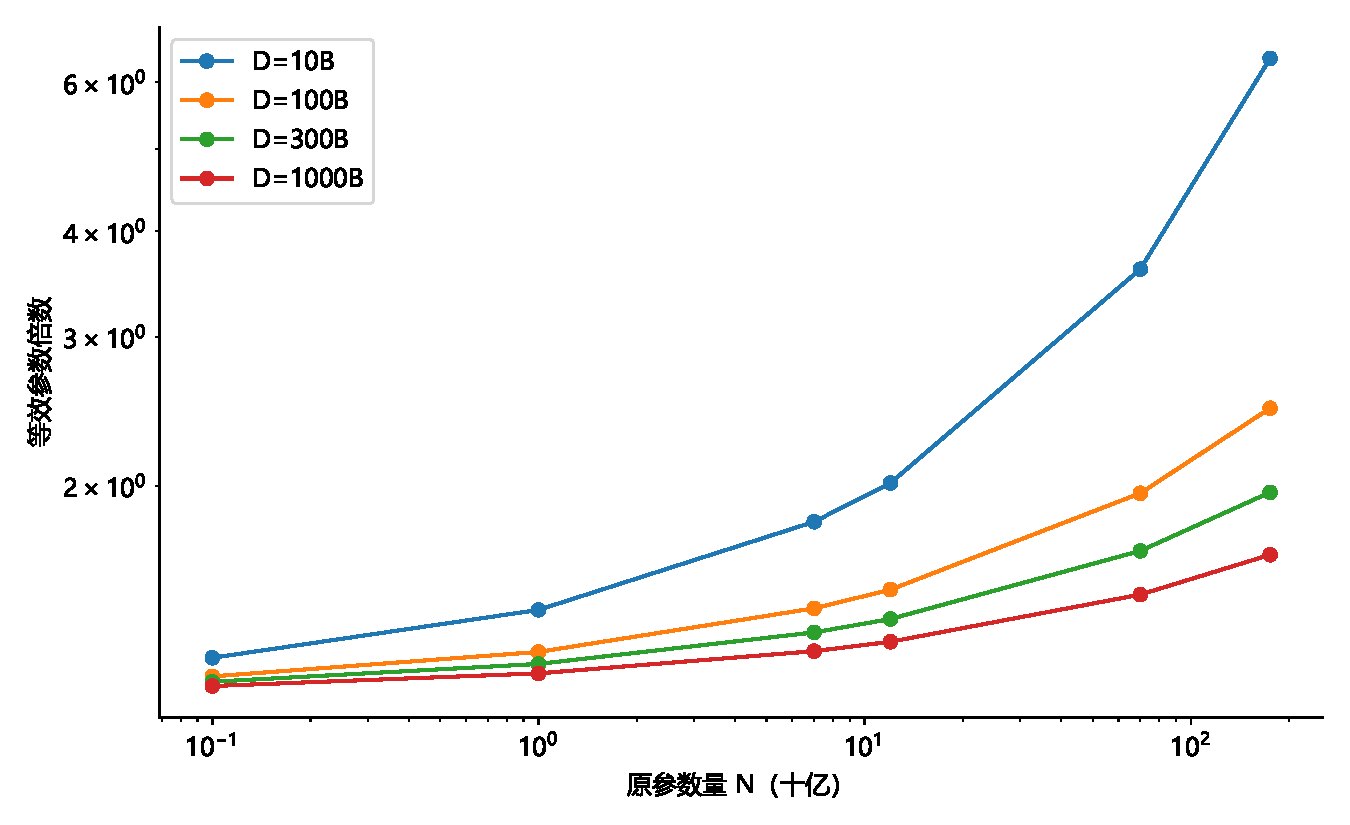
\includegraphics[width=\linewidth]{figures/q2_fig03_quality_parameter_equivalence.pdf}
         \caption{质量提高 0.1 的等效参数扩容倍数（$\kappa=1$）}
         \label{fig:p2_equiv}
        \end{figure}

        \subsubsection{领域主效应与组合关系}  % 5.3.6
        取 $N=7$B、$D=300$B、$\bm p=\bm p_0$，沿常规质量路径计算领域效应。
        
        dm\_mathematics、ubuntu\_irc 和 stackexchange 领域的方向导数分别为 $-0.116345$、$-0.099070$ 和 $-0.020586$。例如，在足够小且可行的邻域内，dm\_mathematics 领域份额增加一个百分点对应的损失变化约为 $-0.001163$。这些数值描述指定让出方式下的局部效应，不能直接推断大幅改变配方的收益。
        
        图\ref{fig:p2_interaction}给出各领域对的结果。enron\_emails 与 europarl 的混合导数为 $-6.861304$，表现为局部互补；philpapers 与 enron\_emails 的混合导数为 $32.483430$，表现为局部替代。不过，交互符号本身不能证明同时增加两个领域就能改善性能，还必须结合各自的一阶效应。低占比领域的结果尤其依赖参考配方及扰动方式，故这些关系不解释为普适因果关系。
        
        \begin{figure}[H]
         \centering
         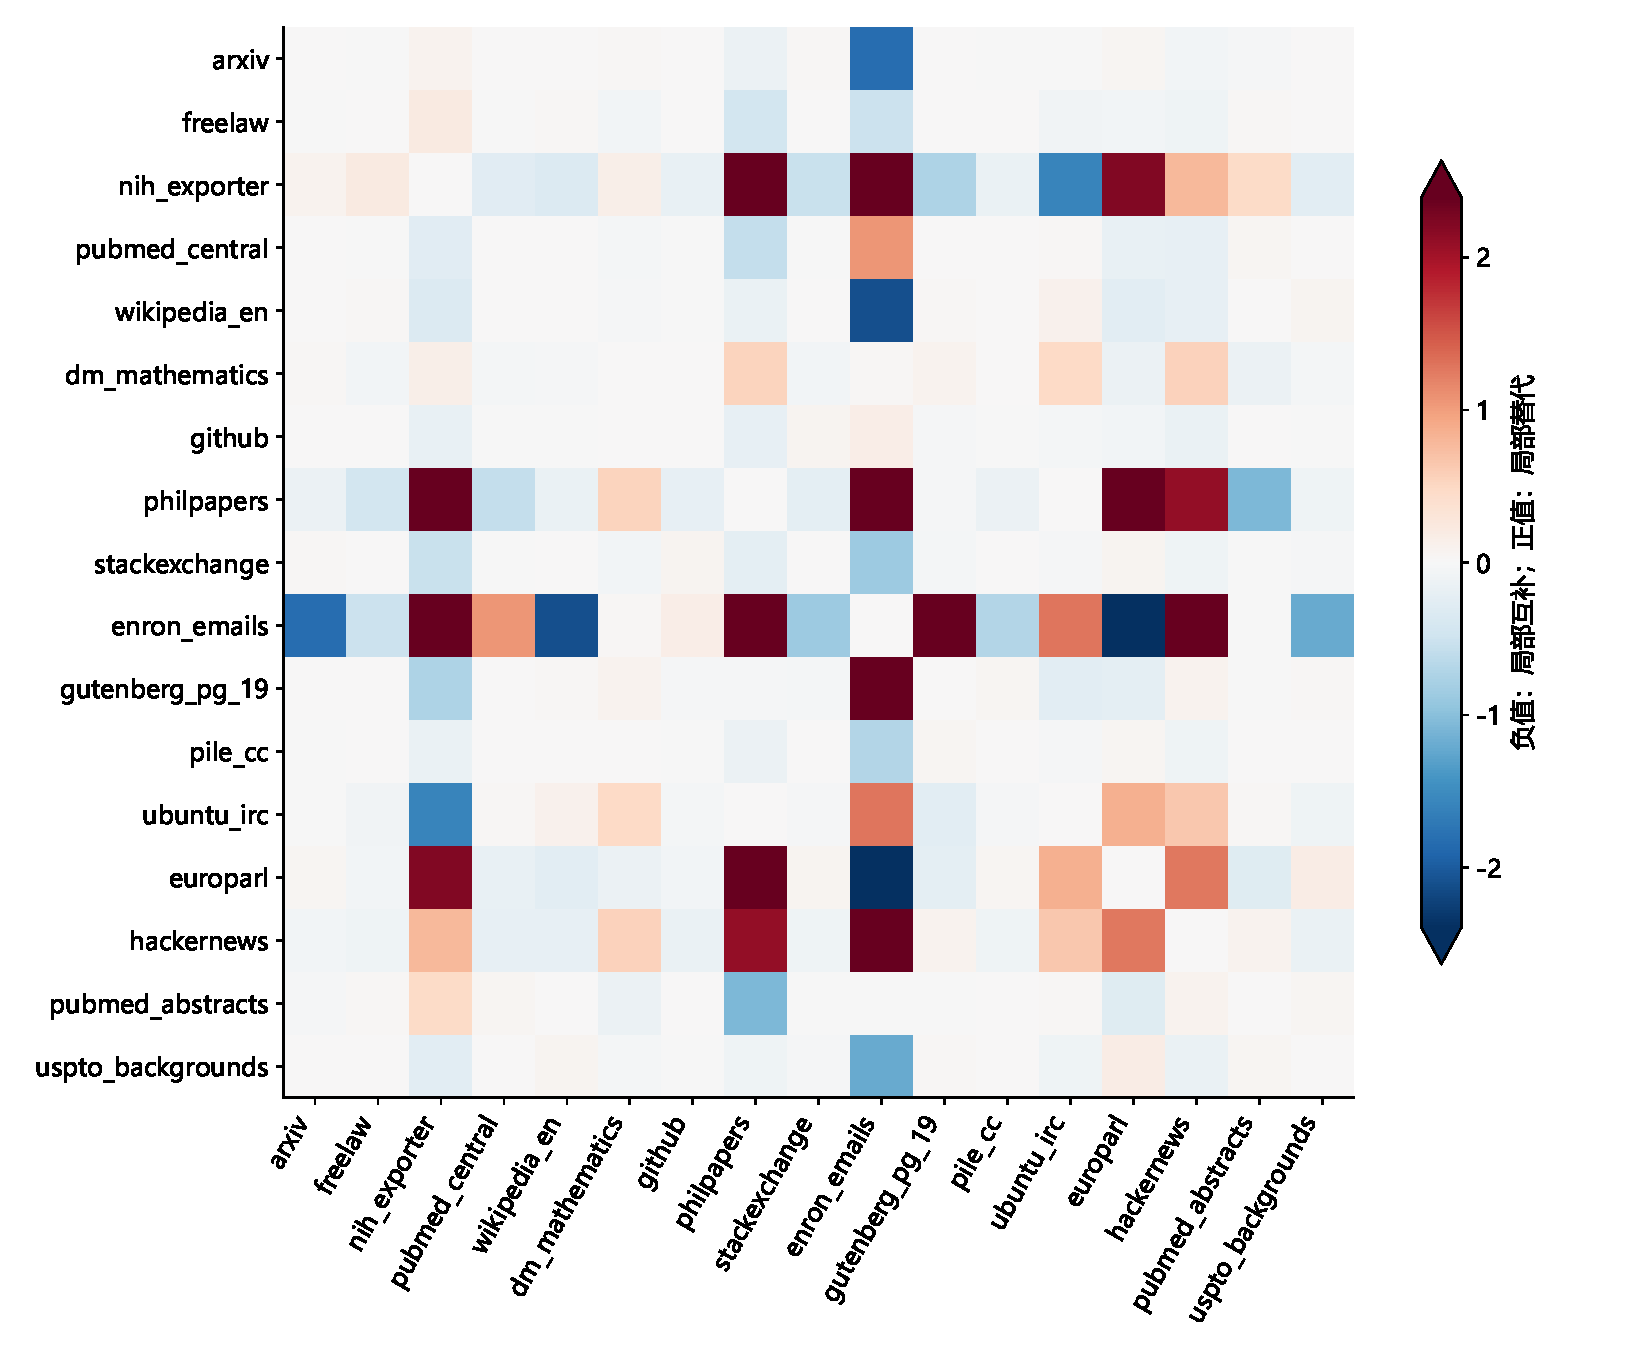
\includegraphics[width=\linewidth]{figures/q2_fig04_domain_interactions.pdf}
         \caption{常规质量路径下的领域局部交互}
         \label{fig:p2_interaction}
        \end{figure}
        
        \subsubsection{质量尺度与配比迁移的敏感性}  % 5.3.7
        质量量尺换算是资源替代结论的重要不确定性。保持式\eqref{eq:p2_example}的其他条件，将 $\kappa$ 分别取为 0.5、1 和 2，得到表\ref{tab:p2_sensitivity}。等效扩容比例由 15.66\% 变为 83.97\%，变化幅度明显大于固定模型下的 Bootstrap 区间。因此，34.35\% 应解释为主情景估计，而不是不依赖质量定义的固定比例。
        
        \begin{table}[H]
         \centering
         \caption{质量量尺对等效扩容结果的影响}
         \label{tab:p2_sensitivity}
         \begin{tabular}{ccc}
          \toprule
          质量尺度 $\kappa$ & 等效参数量 / B & 相对原 7B 的扩容比例 \\
          \midrule
          0.5 & 8.095896 & 15.66\% \\
          1.0 & 9.404464 & 34.35\% \\
          2.0 & 12.877917 & 83.97\% \\
          \bottomrule
         \end{tabular}
        \end{table}
        
        对配比迁移，比较各配方的 13 域平均损失排序，在 1M、60M、1B 检验集上的 Spearman 相关系数分别为 0.689、0.660 和 0.492；在估算的 10B、70B 配方表中则分别为 $-0.599$ 和 $-0.675$，尚不支持大规模下保持相同排序的结论。这里评价的是 13 个验证领域平均 Loss 的排序，与问题一逐验证域计算相关系数再取平均的指标不同。此外，沿常规质量路径，任意正 $\lambda_p$ 都保留同样的配方排序，故排序成绩不能用于唯一确定迁移幅度。

        \subsubsection{大模型外推的适用边界}  % 5.3.8
        B1 支持的参数量范围约为 0.070542B 至 11.965825B，数据量范围为 0.134B 至 299.893B tokens。B9、B10 所涉及的大模型在质量与配比缺失时，采用参考条件进行情景计算，其结果不作为实测精度结论。本文给出的广义标度律能够在明确假设下统一计算规模、质量和配比的作用，并为后续资源配置提供边际收益与替代条件；其跨来源强度及大规模适用性仍需统一验证口径下的联合训练实验进一步检验。

        \subsubsection{小结}  % 5.3.9
        本问将问题一的配方响应与附件 B 的规模信息衔接，得到同时包含参数量、数据量、质量和领域配比的广义标度律。分阶段估计得到参数指数 $\widehat\alpha=0.339921$、数据指数 $\widehat\beta=0.279796$ 和质量响应 $\widehat\gamma=0.410160$。质量项在 B6 半合成数据的分组验证中降低预测误差，但 B8 的方向冲突表明该规律存在明确的来源边界。

        在 7B 参数、300B tokens 的主情景下，质量提高 0.1 约等效于扩容至 9.404B；这一结果受质量量尺假设影响，不能直接转换为固定的经济收益。领域边际和交互关系仅表示参考配方邻域内的模型响应。上述估计、条件与不确定性共同构成后续资源配置分析的输入。
        
\section{问题三}   % 6
    \subsection{问题分析}

    \subsection{模型建立}

    \subsection{建模结果}

\section{问题四}   % 7
    \subsection{问题分析}

    \subsection{模型建立}

    \subsection{建模结果}

\section{模型评价}  % 8 (1~3 pages)
模型评价


\begin{thebibliography}{99}  % 参考文献
 \bibitem{wettig2024qurating} Wettig, A., Gupta, A., Malik, S., Chen, D. 2024. QuRating: Selecting High-Quality Data for Training Language Models. Proceedings of the 41st International Conference on Machine Learning, PMLR, 235, 52915--52971. \url{https://proceedings.mlr.press/v235/wettig24a.html}. \bibitem{huber1964robust} Huber, P. J. 1964. Robust Estimation of a Location Parameter. The Annals of Mathematical Statistics, 35(1), 73--101. \url{https://doi.org/10.1214/aoms/1177703732}. \bibitem{aitchison1982compositional} Aitchison, J. 1982. The Statistical Analysis of Compositional Data. Journal of the Royal Statistical Society. Series B (Methodological), 44(2), 139--177. \url{https://doi.org/10.1111/j.2517-6161.1982.tb01195.x}. \bibitem{liu2025regmix} Liu, Q., Zheng, X., Muennighoff, N., Zeng, G., Dou, L., Pang, T., Jiang, J., Lin, M. 2025. RegMix: Data Mixture as Regression for Language Model Pre-training. The Thirteenth International Conference on Learning Representations (ICLR). \url{https://arxiv.org/abs/2407.01492}. \bibitem{egozcue2003ilr} Egozcue, J. J., Pawlowsky-Glahn, V., Mateu-Figueras, G., Barcel\'o-Vidal, C. 2003. Isometric Logratio Transformations for Compositional Data Analysis. Mathematical Geology, 35(3), 279--300. \url{https://doi.org/10.1023/A:1023818214614}. \bibitem{hoerl1970ridge} Hoerl, A. E., Kennard, R. W. 1970. Ridge Regression: Biased Estimation for Nonorthogonal Problems. Technometrics, 12(1), 55--67. \url{https://doi.org/10.1080/00401706.1970.10488634}. \bibitem{diakoulaki1995critic} Diakoulaki, D., Mavrotas, G., Papayannakis, L. 1995. Determining objective weights in multiple criteria problems: The CRITIC method. Computers \& Operations Research, 22(7), 763--770. \url{https://doi.org/10.1016/0305-0548(94)00059-H}.
 
\bibitem{hoffmann2022chinchilla} Hoffmann, J., Borgeaud, S., Mensch, A., et al. 2022. An empirical analysis of compute-optimal large language model training. Advances in Neural Information Processing Systems, 35. \url{https://proceedings.neurips.cc/paper_files/paper/2022/hash/c1e2faff6f588870935f114ebe04a3e5-Abstract.html}. \bibitem{ye2025mixing} Ye, J., Liu, P., Sun, T., Zhan, J., Zhou, Y., Qiu, X. 2025. Data Mixing Laws: Optimizing Data Mixtures by Predicting Language Modeling Performance. The Thirteenth International Conference on Learning Representations (ICLR). \url{https://arxiv.org/abs/2403.16952}. \bibitem{biderman2023pythia} Biderman, S., Schoelkopf, H., Anthony, Q. G., et al. 2023. Pythia: A Suite for Analyzing Large Language Models Across Training and Scaling. Proceedings of the 40th International Conference on Machine Learning, PMLR, 202, 2397--2430. \url{https://proceedings.mlr.press/v202/biderman23a.html}. \bibitem{subramanyam2026quality} Subramanyam, A., Chen, Y., Grossman, R. L. 2026. Scaling Laws Revisited: Modeling the Role of Data Quality in Language Model Pretraining. The Fourteenth International Conference on Learning Representations (ICLR). \url{https://arxiv.org/abs/2510.03313}. \bibitem{virtanen2020scipy} Virtanen, P., Gommers, R., Oliphant, T. E., et al. 2020. SciPy 1.0: Fundamental Algorithms for Scientific Computing in Python. Nature Methods, 17(3), 261--272. \url{https://doi.org/10.1038/s41592-019-0686-2}. \bibitem{efron1979bootstrap} Efron, B. 1979. Bootstrap Methods: Another Look at the Jackknife. The Annals of Statistics, 7(1), 1--26. \url{https://doi.org/10.1214/aos/1176344552}. \end{thebibliography}


\clearpage


\begin{appendices}  % 附录
    % \setcounter{page}{1}  % 如果需要可以自行重置页码。
    \section{MATLAB 源程序}    % 附录 A
    \renewcommand{\thesubsection}{A\thinskip.\thinskip\arabic{subsection}}
        \subsection{第1问程序}  % A.1
        \vspace{-2ex}
        
        \begin{Matlab}{code.m}
        clear all
        kk=2;
        [mdd,ndd]=size(dd);
        while ~isempty(V)
            [tmpd,j]=min(W(i,V));
            tmpj=V(j);
            for k=2:ndd
                [tmp1,jj]=min(dd(1,k)+W(dd(2,k),V));
                tmp2=V(jj);
                tt(k-1,:)=[tmp1,tmp2,jj];
            end
            tmp=[tmpd,tmpj,j;tt];
            [tmp3,tmp4]=min(tmp(:,1));
            if tmp3==tmpd,
                ss(1:2,kk)=[i;tmp(tmp4,2)];
            else
                tmp5=find(ss(:,tmp4)~=0);
                tmp6=length(tmp5);
                if dd(2,tmp4)==ss(tmp6,tmp4)
                    ss(1:tmp6+1,kk)=[ss(tmp5,tmp4);tmp(tmp4,2)];
                else, ss(1:3,kk)=[i;dd(2,tmp4);tmp(tmp4,2)];
                end
            end
            dd=[dd,[tmp3;tmp(tmp4,2)]];
            V(tmp(tmp4,3))=[];
            [mdd,ndd]=size(dd);kk=kk+1;
        end;
        S=ss; D=dd(1,:);
        \end{Matlab}
        \vspace{2ex}
    
    \clearpage
    \section{Python 源程序}    % 附录 B
    \renewcommand{\thesubsection}{B\thinskip.\thinskip\arabic{subsection}}
        \subsection{第2问程序}  % B.1
        \vspace{-2ex}
        \begin{Python}{mip1.py}
        # This example formulates and solves the following  MIP model:
        #  maximize
        #        x +   y + 2 z
        #  subject to
        #        x + 2 y + 3 z <= 4
        #        x +   y       >= 1
        #        x, y, z binary
        
        # import gurobipy as gp
        from gurobipy import * #GRB
        try:
            # Create a new model
            m = Model("mip1")
            # Create variables
            x = m.addVar(vtype=GRB.BINARY, name="x")
            y = m.addVar(vtype=GRB.BINARY, name="y")
            z = m.addVar(vtype=GRB.BINARY, name="z")
            # Set objective
            m.setObjective(x + y + 2 * z, GRB.MAXIMIZE)
            # Add constraint: x + 2 y + 3 z <= 4
            m.addConstr(x + 2 * y + 3 * z <= 4, "c0")
            # Add constraint: x + y >= 1
            m.addConstr(x + y >= 1, "c1")
            # Optimize model
            m.optimize()
            for v in m.getVars():
                print('%s %g' % (v.varName, v.x))
            print('Obj: %g' % m.objVal)
        
        except GurobiError as e:
            print('Error code ' + str(e.errno) + ': ' + str(e))
        
        except AttributeError:
            print('Encountered an attribute error')
        \end{Python}
    
\end{appendices}


\end{document} 